\documentclass{beamer}\usepackage[]{graphicx}\usepackage[]{color}
%% maxwidth is the original width if it is less than linewidth
%% otherwise use linewidth (to make sure the graphics do not exceed the margin)
\makeatletter
\def\maxwidth{ %
  \ifdim\Gin@nat@width>\linewidth
    \linewidth
  \else
    \Gin@nat@width
  \fi
}
\makeatother

\definecolor{fgcolor}{rgb}{0.345, 0.345, 0.345}
\newcommand{\hlnum}[1]{\textcolor[rgb]{0.686,0.059,0.569}{#1}}%
\newcommand{\hlstr}[1]{\textcolor[rgb]{0.192,0.494,0.8}{#1}}%
\newcommand{\hlcom}[1]{\textcolor[rgb]{0.678,0.584,0.686}{\textit{#1}}}%
\newcommand{\hlopt}[1]{\textcolor[rgb]{0,0,0}{#1}}%
\newcommand{\hlstd}[1]{\textcolor[rgb]{0.345,0.345,0.345}{#1}}%
\newcommand{\hlkwa}[1]{\textcolor[rgb]{0.161,0.373,0.58}{\textbf{#1}}}%
\newcommand{\hlkwb}[1]{\textcolor[rgb]{0.69,0.353,0.396}{#1}}%
\newcommand{\hlkwc}[1]{\textcolor[rgb]{0.333,0.667,0.333}{#1}}%
\newcommand{\hlkwd}[1]{\textcolor[rgb]{0.737,0.353,0.396}{\textbf{#1}}}%
\let\hlipl\hlkwb

\usepackage{framed}
\makeatletter
\newenvironment{kframe}{%
 \def\at@end@of@kframe{}%
 \ifinner\ifhmode%
  \def\at@end@of@kframe{\end{minipage}}%
  \begin{minipage}{\columnwidth}%
 \fi\fi%
 \def\FrameCommand##1{\hskip\@totalleftmargin \hskip-\fboxsep
 \colorbox{shadecolor}{##1}\hskip-\fboxsep
     % There is no \\@totalrightmargin, so:
     \hskip-\linewidth \hskip-\@totalleftmargin \hskip\columnwidth}%
 \MakeFramed {\advance\hsize-\width
   \@totalleftmargin\z@ \linewidth\hsize
   \@setminipage}}%
 {\par\unskip\endMakeFramed%
 \at@end@of@kframe}
\makeatother

\definecolor{shadecolor}{rgb}{.97, .97, .97}
\definecolor{messagecolor}{rgb}{0, 0, 0}
\definecolor{warningcolor}{rgb}{1, 0, 1}
\definecolor{errorcolor}{rgb}{1, 0, 0}
\newenvironment{knitrout}{}{} % an empty environment to be redefined in TeX

\usepackage{alltt}

\def\currentCourse{An introduction to graph analysis and modeling}
\def\currentInstitute{MSc in Statistics for Smart Data -- ENSAI}
\def\currentLogo{../common_figs/logo_ensai}
\def\currentDate{Automn semester, 2018}
\def\currentChapter{The Stochastic block model}


% THEME BEAMER
\usepackage{../beamer_theme}

\graphicspath{{figures/},{../common_figs/}}

\usepackage{multirow}
\usepackage{tikz}
\usepackage[vlined]{algorithm2e}

\pgfdeclareimage[width=.5cm]{computer}{computer.png}

% \usetikzlibrary{calc,shapes,backgrounds,arrows,automata,shadows,positioning}
% \tikzstyle{every state}=[fill=red,draw=none,scale=0.7,font=\small,text=white]
% \tikzstyle{every edge}=[-,shorten >=1pt,auto,thin,draw]
% \tikzstyle{alertstate}=[fill=bleu]
% \definecolor{genecolor}{RGB}{94,135,173}

\title{\currentCourse}

\subtitle{\huge\currentChapter\normalsize}

\institute{\currentInstitute}

\date{\currentDate}



\AtBeginSection{
  \begin{frame}<beamer>
    \frametitle{Outline}
    \framesubtitle{\insertpart}
    \tableofcontents[currentsection,currentsubsection, subsectionstyle=show/shaded/hide]  
  \end{frame}
}

\AtBeginSubsection{
  \begin{frame}<beamer>
    \frametitle{Outline}
    \framesubtitle{\insertpart}
    \tableofcontents[currentsection,currentsubsection, subsectionstyle=show/shaded/hide]  
  \end{frame}
}

\AtBeginSubsubsection{
  \begin{frame}<beamer>
    \frametitle{Outline}
    \framesubtitle{\insertpart}
    \tableofcontents[currentsection,currentsubsection, subsectionstyle=show/shaded/hide]  
  \end{frame}
}

\newcommand{\dotitlepage}{%
  \begin{frame}
    \titlepage
    \vfill
    \begin{center}
        \scriptsize\url{https://github.com/jchiquet/CourseStatNetwork}
    \end{center}
    \vfill
    \includegraphics[width=2cm]{\currentLogo}\hfill
    
\includegraphics[width=2.5cm]{logo_inra}
  \end{frame}
  %
}

\newcommand{\dotoc}{%
  \begin{frame}
    \frametitle{Outline}
    \tableofcontents[currentsection,
    sectionstyle=show/show,
    subsectionstyle=hide]
  \end{frame}
  %
}



\usetikzlibrary{calc,shapes,backgrounds,arrows,automata,shadows,positioning}
\IfFileExists{upquote.sty}{\usepackage{upquote}}{}
\begin{document}

\dotitlepage

\begin{frame}
  \frametitle{Motivations}

  \begin{block}{Last time: \alert{find an underlying organization in a observed network}}
    Spectral or hierachical clustering for network data \\
    \begin{itemize}
      \item[$\rightsquigarrow$] \alert{Not model-based}, thus no statistical inference possible
    \end{itemize}
  \end{block}

  \begin{block}{Today: \alert{clustering of network based on a probabilistic model of the graph}}<2->
    Become familiar with
    \begin{itemize}
      \item the stochastic block model, a random graph model tailored for clustering vertices,
      \item the variational EM algorithm used to infer SBM from network data.
    \end{itemize}
  \end{block}

  \onslide<3>{
  \begin{center}
    hierarchical clustering $\leftrightarrow$ \alert{Gaussian mixture models} \\
      $\Updownarrow$ \\
    hierarchical/spectral clustering for network $\leftrightarrow$ Stochastic block model
  \end{center}
  }

\end{frame}

\begin{frame}
  \frametitle{Outline}
  \tableofcontents
\end{frame}

%% ==========================================================================
\section{Background: mixture models and EM}
%% ==========================================================================

\begin{frame}
  \frametitle{References}

    \begin{thebibliography}{99}
      \setbeamertemplate{bibliography item}[book]

    \bibitem[EK2]{EK2} Pattern recognition and machine learning,
    \newblock \textcolor{black}{Christopher Bishop}
    \newblock \alert{Chapter 9: Mixture Models and EM}
    \newblock {\tiny\url{http://users.isr.ist.utl.pt/~wurmd/Livros/school/}}

    \bibitem[SR]{SR} Models with Hidden Structure with Applications in Biology and Genomics,
    \newblock \textcolor{black}{Stéphane Robin}
    \newblock \alert{Master MathSV Course}
    \newblock {\tiny\url{https://www6.inra.fr/mia-paris/content/download/4587/42934/version/1/file/ModelsHiddenStruct-Biology.pdf}}

      \setbeamertemplate{bibliography item}[article]

    \bibitem[CM1]{CM1} Classification non-supervisées,
    \newblock \textcolor{black}{É. Lebarbier, T. Mary-Huard}
    \newblock \alert{Chapitre 3 - méthode probabiliste: le modèle de mélange}
    \newblock {\tiny\url{https://www.agroparistech.fr/IMG/pdf/ClassificationNonSupervisee-AgroParisTech.pdf}}

    \end{thebibliography}


\end{frame}

%% ==========================================================================
\subsection{Mixture models}
%% ==========================================================================

\begin{frame}
  \frametitle{Latent variables models}

  \begin{definition}
    A \alert{latent variable model} is a statistical model that relates, for $i=1,\dots,n$ individuals,
  \begin{itemize}
    \item a set of \alert{manifest} (observed) variables $\bX = (X_i, i=1,\dots,n)$ to
    \item a set of \alert{latent} (unobserved) variables $\bZ = (Z_i, i=1,\dots,n)$.
    \end{itemize}
  \end{definition}

  \begin{block}{Common assumption: conditional independence}
    \vspace{-.5cm}
    \begin{equation*}
      \prob((X_1, \dots, X_n)|(Z_1,\dots, Z_n))  = \prod_{i=1}^n \prob(X_i| Z_i).
    \end{equation*}
  \end{block}

  \vspace{-.25cm}

  \begin{block}{Famous examples}<2->
    \vspace{-.25cm}
    \begin{itemize}
      \item $(Z_i, i\geq 1)$ is Markov chain: \alert{Markov models}
      \item $Z_i$ categorical and independent: \alert{mixture models}
      \item<3> \alert{what if $X_i = X_{i'j'}$ is a collection of edges in a graph?}
    \end{itemize}
  \end{block}

\end{frame}

\begin{frame}
  \frametitle{Mixture models: the latent variables}

    When $(Z_1,\dots,Z_n)$ are independent categorical variables, they give a \alert{natural (latent) classification of the observations} $(X_1,\dots,X_n)$ -- or \alert{labels}.

  \begin{block}{Notations}<2->
    Let $(Z_1, \dots, Z_n)$ be \textit{iid} categorical variables with distribution
    \vspace{-.25cm}
    \begin{equation*}
      \prob(i \in q) = \prob(Z_i = q) = \alpha_q, \quad \text{s.t.}  \sum_{q=1}^Q \alpha_q = 1.
    \end{equation*}
  \end{block}

  \vspace{-.5cm}
  \begin{block}{Alternative (equivalent) notation}<3>
    Let $Z_i=(Z_{i1},\dots, Z_{iq})$ be an indicator vector of label for $i$:
    \vspace{-.25cm}
    \begin{equation*}
      \prob(i \in q) = \prob(Z_{iq}  =  1)=\alpha_q,  \quad  \text{s.t.} \sum_{q=1}^Q \alpha_q = 1.
    \end{equation*}
    By definition, $Z_i \sim \mathcal{M}(1, \balpha)$, with $\balpha = (\alpha_1, \dots, \alpha_Q)$.
  \end{block}

\end{frame}

\begin{frame}
  \frametitle{Mixture models: the manifest variables}

  A mixture model represents the \alert{presence of subpopulations} within an overall population as follows:
  \begin{equation*}
    \prob(X_i) = \sum_{z_i \in \mathcal{Z}_i} \prob(X_i , Z_i) = \sum_{Z_i \in \mathcal{Z}_i}\prob(X_i | Z_i) \prob(Z_i).
  \end{equation*}

  \vfill

  \begin{block}{Conditional distribution of the manifest variables}
    We assume a \alert{parametric distribution} of $X$ in each subpopulation
    \begin{equation*}
      X_i | \set{Z_i = q} \sim \prob_{\theta_q} \qquad \bigg(\Leftrightarrow X_i | \set{Z_{iq}} = 1 \sim \prob_{\theta_q}\bigg)
    \end{equation*}
    The specificity of each class is handled by $\set{\btheta_q}_{q=1}^Q$.
  \end{block}

\end{frame}

\begin{frame}
  \frametitle{Mixture models: likelihoods}

  \begin{block}{The complete-data likelihood}
    It is the join distribution of $(X_i,Z_i)$:
    \begin{equation*}
      \prob(X_i,Z_i) = \alpha_{Z_i} \prob_{\btheta_q}(X_{Z_i})
    \end{equation*}
  \end{block}

  \vspace{-.25cm}

  \begin{block}{The incomplete-data likelihood}<2>
    It is the marginal distribution of $X_i$ once $Z_i$ integrated:
    \begin{equation*}
      \prob(X_i) = \sum_{q=1}^Q \prob(X_i, Z_i = q)  = \sum_{q=1}^Q \alpha_q \prob_{\btheta_q}(X_i)
    \end{equation*}
  \end{block}

  \vspace{-.25cm}

  \onslide<2>{
    $\rightsquigarrow$ A \alert{mixture model} is a sum of distributions weigthed by the proportion of each subpopulation.
  }

\end{frame}

%% ==========================================================================
\subsection{Expectation-Maximization algorithm}
%% ==========================================================================

\begin{frame}
  \frametitle{Intractability of the Likelihood}

  \begin{block}{Maximum Likelihood Estimator}
    The MLE aims to maximize the (marginal) likehood of the observations:
    \begin{equation*}
      L(\btheta; \bX) = \prob_{\btheta}((X_1,\dots,X_n)) = \int_{\bZ \in \mathcal{Z}} \prob_{\btheta}(\bX,\bZ) \mathrm{d} \bZ
    \end{equation*}
    Integrations are summation over $\set{1,\dots,Q}$: we have $Q^n$ terms !
  \end{block}

  \vfill

  \begin{block}{Intractable summation}<2->
    With mixture models, for $\btheta = (\btheta_1,\dots,\btheta_Q)$ we have
    \begin{equation*}
      \log L(\btheta; \bX) = \sum_{i=1}^n \log \set{\sum_{q=1}^Q \alpha_q \prob_{\btheta_q}(X_i)}.
    \end{equation*}
    \alert{$\rightsquigarrow$ Direct maximization of the likelihood is impossible in practice}
  \end{block}

\end{frame}

\begin{frame}
  \frametitle{Bayes decision rule / Maximum \textit{a posteriori}}

  \begin{block}{Principle}
    Affect an individual $i$ to the subpopulation which is the most likely according to the data:
    \begin{equation*}
      \tau_{iq} = \prob(Z_{iq}=1 | X_i = x_i)
    \end{equation*}
    This is the \alert{posterior probability} for $i\in q$.
  \end{block}

  \vfill

  \begin{block}{Application of the Bayes Theorem}
    It is straightforward to show that
    \begin{equation*}
      \tau_{iq} = \frac{\alpha_q \prob_{\theta_q}(x_i)}{\sum_{q=1}^Q \alpha_q \prob_{\theta_q}(x_i)}
    \end{equation*}
  \end{block}

\end{frame}

\begin{frame}
  \frametitle{Principle of the EM algorithm}

  \begin{block}{If $\btheta$ were known}
    \dots estimating the \alert{posterior probability $\prob(Z_i|\bX)$} of $\bZ$ should be easy\\
    \textit{By means of the Bayes decision rule}
  \end{block}

  \vfill

  \begin{block}{If $\bZ$ were known\dots}
    \dots estimating the \alert{best set of parameter} $\btheta$ should be easy\\
    \textit{This is close to usual maximum likelihood estimation}
  \end{block}

  \vfill

  \begin{block}{EM principle}<2>
    Maximize the marginal likelihood iteratively:
    \begin{enumerate}
      \item Initialize $\btheta$
      \item Compute the probability of $\bZ$ given $\btheta$
      \item Get a better $\btheta$ with the new $\bZ$
      \item Iterate until convergence
    \end{enumerate}
  \end{block}


\end{frame}

\begin{frame}
  \frametitle{Formal algorithm}

  \begin{block}{Initialization: \textcolor{black}{start from a good guess either of $\bZ$ or $\btheta$, then iterate 1-2}}
  \end{block}

  \begin{block}{1. Expectation step}
    Calculate the expected value of the loglikelihood under the current $\btheta$
    \begin{equation*}
      Q\left(\btheta|\btheta^{(t)}\right) = \E_{\bZ|\bX;\btheta^{(t)}}\big[ \log L (\btheta;\bX,\bZ)  \big] \qquad (\textit {needs } \prob_{\btheta^{(t)}}(\bZ|\bX))
    \end{equation*}
  \end{block}

  \vfill

  \begin{block}{2. Maximization step}
    Find the parameters that maximize this quantity
    \begin{equation*}
      \btheta^{(t+1)} = \argmax_{\btheta} Q\left(\btheta|\btheta^{(t)}\right)
    \end{equation*}
  \end{block}

  Stop when $\|\btheta^{(t+1)} - \btheta^{(t)}\| < \varepsilon$ or $\|Q^{(t+1)} - Q^{(t)}\| < \varepsilon$

\end{frame}

\begin{frame}
  \frametitle{(Basic) Convergence analysis}

  \begin{theorem}
    At each step of the EM algorithm, the loglikelihood increases. EM thus reaches a local optimum.
  \end{theorem}

  \begin{proof}
    On board.
  \end{proof}

\end{frame}

\begin{frame}
  \frametitle{Choosing the number of component}

  \begin{block}{Reminder: Bayesian Information Criterion}
    The BIC is a model selection criterion which penalizes the adjustement to the data by the number of parameter in model $\mathcal{M}$ as follows:
    \begin{equation*}
      \mathrm{BIC}(\mathcal{M}) = \log L(\hatbtheta; \bX) - \frac{1}{2}\log(n) \mathrm{df}(\mathcal{M}).
    \end{equation*}
  \end{block}

  \vspace{-.35cm}

  \begin{block}{Integrated Classification Criterion}<2->
    It is an adaptation working with the complete-data likelihood:
    \vspace{-.25cm}
    \begin{align*}
      \mathrm{ICL}(\mathcal{M}) & = \log L(\hatbtheta; \bX, \hat{\bZ}) + \frac{1}{2}\log(n) \mathrm{df}(\mathcal{M}) \\
      & = \mathrm{BIC} - \mathcal{H}(\prob(\hat \bZ | \bX),
    \end{align*}
    where the entropy $\mathcal{H}$ measures the separability of the subpopulations.
  \end{block}

  \vfill

  \onslide<3>{$\rightsquigarrow$ \alert{We choose $\mathcal{M}(Q)$ that maximizes either BIC or ICL}}
\end{frame}

%% ==========================================================================
\subsection{Example: mixture of Gaussians}
%% ==========================================================================

\begin{frame}
  \frametitle{Mixture of Gaussians}
  \framesubtitle{Calculs in the univariate case: complete likelihood}

  The distribution of $X_i$ conditional on the label of $i$ is assumed to be a univariate Gaussian distribution with unknown parameters:
  \begin{equation*}
  X_i | Z_{iq} = 1 \sim \mathcal{N}(\mu_q,\sigma^2_q)
  \end{equation*}

  \begin{block}{complete Likelihood $(\bX,\bZ)$}
  The model complete loglikelihood is
    \begin{multline*}
        \log L(\boldsymbol{\mu},\boldsymbol{\sigma}^2; \bX, \bZ)  = \\ \sum_{i=1}^n \sum_{q=1}^Q Z_{iq} \left(\log \alpha_q - \log\sigma_q -\log(\sqrt{2\pi}) - \frac{1}{2\sigma_q^2} (x_i - \mu_q)^2 \right)
   \end{multline*}
  \end{block}

\end{frame}

\begin{frame}
  \frametitle{Mixture of Gaussians}
  \framesubtitle{Calculs in the univariate case: E-step}

  \begin{block}{E-step}
    For fixed values of  $\mu_q, \sigma_q^2$ and  $\alpha_q$, the  estimates of  the
  posterior probabilities $\hat\tau_{iq}= \P(Z_{iq}=1|X_i)$ are
    \begin{equation*}
        \hat\tau_{iq} = \frac{\alpha_q \mathcal{N}(x_i; {\mu}_q, \sigma_q^2)}{\sum_{q=1}^Q \alpha_q \mathcal{N}(x_i; {\mu}_q, \sigma_q^2)},
   \end{equation*}
   where $\mathcal{N}$ is the density of the normal distribution.
  \end{block}

\end{frame}

\begin{frame}
  \frametitle{Mixture of Gaussians}
  \framesubtitle{Calculs in the univariate case: M-step}

  \begin{block}{M-step}
    For fixed values of  $\tau_{iq}$, the  estimates of  the model parameters are
    \begin{equation*}
    \hat\alpha_q = \frac{\sum_{i=1}^n \tau_{iq}}{\sum_{i=1}^n\sum_{q=1}^Q \tau_{iq}} \quad \hat\mu_q = \frac{\sum_i \tau_{iq} x_i}{\sum_i \tau_{iq}} \quad \hat\sigma^2_q = \frac{\sum_{i=1}^n \tau_{iq} (x_i-\mu_q)^2}{\sum_{i=1}^n \tau_{iq}}
   \end{equation*}
  \end{block}

\end{frame}

\begin{frame}[fragile]
  \frametitle{R code: auxiliary functions}

We start by defining functions to compute the complete model loglikelihood, perform the E step and the M step.
\begin{knitrout}\scriptsize
\definecolor{shadecolor}{rgb}{0.969, 0.969, 0.969}\color{fgcolor}\begin{kframe}
\begin{alltt}
\hlstd{get.cloglik} \hlkwb{<-} \hlkwa{function}\hlstd{(}\hlkwc{X}\hlstd{,} \hlkwc{Z}\hlstd{,} \hlkwc{theta}\hlstd{) \{}
  \hlstd{alpha} \hlkwb{<-} \hlstd{theta}\hlopt{$}\hlstd{alpha; mu} \hlkwb{<-} \hlstd{theta}\hlopt{$}\hlstd{mu; sigma} \hlkwb{<-} \hlstd{theta}\hlopt{$}\hlstd{sigma}
  \hlstd{xs} \hlkwb{<-} \hlkwd{scale}\hlstd{(}\hlkwd{matrix}\hlstd{(X,}\hlkwd{length}\hlstd{(x),}\hlkwd{length}\hlstd{(alpha)),mu,sigma)}
  \hlkwd{return}\hlstd{(}\hlkwd{sum}\hlstd{(Z}\hlopt{*}\hlstd{(}\hlkwd{log}\hlstd{(alpha)}\hlopt{-}\hlkwd{log}\hlstd{(sigma)}\hlopt{-}\hlnum{.5}\hlopt{*}\hlstd{(}\hlkwd{log}\hlstd{(}\hlnum{2}\hlopt{*}\hlstd{pi)}\hlopt{+}\hlstd{xs}\hlopt{^}\hlnum{2}\hlstd{))))}
\hlstd{\}}

\hlstd{M.step} \hlkwb{<-} \hlkwa{function}\hlstd{(}\hlkwc{X}\hlstd{,} \hlkwc{tau}\hlstd{) \{}
  \hlstd{n} \hlkwb{<-} \hlkwd{length}\hlstd{(X); Q} \hlkwb{<-} \hlkwd{ncol}\hlstd{(tau)}
  \hlstd{alpha}  \hlkwb{<-} \hlkwd{colMeans}\hlstd{(tau)}
  \hlstd{mu}     \hlkwb{<-} \hlkwd{colMeans}\hlstd{(tau} \hlopt{*} \hlkwd{matrix}\hlstd{(X,n,Q))} \hlopt{/} \hlstd{alpha}
  \hlstd{sigma}  \hlkwb{<-} \hlkwd{sqrt}\hlstd{(}\hlkwd{colMeans}\hlstd{(tau}\hlopt{*}\hlkwd{sweep}\hlstd{(}\hlkwd{matrix}\hlstd{(X,n,Q),}\hlnum{2}\hlstd{,mu,}\hlstr{"-"}\hlstd{)}\hlopt{^}\hlnum{2}\hlstd{)}\hlopt{/}\hlstd{alpha)}
  \hlkwd{return}\hlstd{(}\hlkwd{list}\hlstd{(}\hlkwc{alpha}\hlstd{=alpha,} \hlkwc{mu}\hlstd{=mu,} \hlkwc{sigma}\hlstd{=sigma))}
\hlstd{\}}

\hlstd{E.step} \hlkwb{<-} \hlkwa{function}\hlstd{(}\hlkwc{X}\hlstd{,} \hlkwc{theta}\hlstd{) \{}
  \hlstd{tau} \hlkwb{<-} \hlkwd{mapply}\hlstd{(}\hlkwa{function}\hlstd{(}\hlkwc{alpha}\hlstd{,} \hlkwc{mu}\hlstd{,} \hlkwc{sigma}\hlstd{) \{}
      \hlstd{alpha}\hlopt{*}\hlkwd{dnorm}\hlstd{(X,mu,sigma)}
    \hlstd{\}, theta}\hlopt{$}\hlstd{alpha, theta}\hlopt{$}\hlstd{mu, theta}\hlopt{$}\hlstd{sigma)}
  \hlkwd{return}\hlstd{(tau} \hlopt{/} \hlkwd{rowSums}\hlstd{(tau))}
\hlstd{\}}
\end{alltt}
\end{kframe}
\end{knitrout}

\end{frame}

\begin{frame}[fragile]
  \frametitle{R code: EM for univariate mixture}

\begin{knitrout}\scriptsize
\definecolor{shadecolor}{rgb}{0.969, 0.969, 0.969}\color{fgcolor}\begin{kframe}
\begin{alltt}
\hlstd{EM.mixture} \hlkwb{<-} \hlkwa{function}\hlstd{(}\hlkwc{X}\hlstd{,} \hlkwc{Q}\hlstd{,}
                       \hlkwc{init.cl}\hlstd{=}\hlkwd{sample}\hlstd{(}\hlnum{1}\hlopt{:}\hlstd{Q,n,}\hlkwc{rep}\hlstd{=}\hlnum{TRUE}\hlstd{),} \hlkwc{max.iter}\hlstd{=}\hlnum{100}\hlstd{,} \hlkwc{eps}\hlstd{=}\hlnum{1e-5}\hlstd{) \{}
    \hlstd{n} \hlkwb{<-} \hlkwd{length}\hlstd{(X); tau} \hlkwb{<-} \hlkwd{matrix}\hlstd{(}\hlnum{0}\hlstd{,n,Q); tau[}\hlkwd{cbind}\hlstd{(}\hlnum{1}\hlopt{:}\hlstd{n,init.cl)]} \hlkwb{<-} \hlnum{1}
    \hlstd{Eloglik} \hlkwb{<-} \hlkwd{vector}\hlstd{(}\hlstr{"numeric"}\hlstd{, max.iter)}
    \hlstd{iter} \hlkwb{<-} \hlnum{0}\hlstd{; cond} \hlkwb{<-} \hlnum{FALSE}

    \hlkwa{while} \hlstd{(}\hlopt{!}\hlstd{cond) \{}
        \hlstd{iter} \hlkwb{<-} \hlstd{iter} \hlopt{+} \hlnum{1}
        \hlcom{## M step}
        \hlstd{theta} \hlkwb{<-} \hlkwd{M.step}\hlstd{(X, tau)}
        \hlcom{## E step}
        \hlstd{tau} \hlkwb{<-} \hlkwd{E.step}\hlstd{(X, theta)}
        \hlcom{## check consistency}
        \hlstd{Eloglik[iter]} \hlkwb{<-} \hlkwd{get.cloglik}\hlstd{(X, tau, theta)}
        \hlkwa{if} \hlstd{(iter} \hlopt{>} \hlnum{1}\hlstd{)}
            \hlstd{cond} \hlkwb{<-} \hlstd{(iter}\hlopt{>=}\hlstd{max.iter)} \hlopt{|} \hlstd{Eloglik[iter]}\hlopt{-}\hlstd{Eloglik[iter}\hlopt{-}\hlnum{1}\hlstd{]} \hlopt{<} \hlstd{eps}
    \hlstd{\}}

    \hlkwd{return}\hlstd{(}\hlkwd{list}\hlstd{(}\hlkwc{alpha} \hlstd{= theta}\hlopt{$}\hlstd{alpha,}  \hlkwc{mu} \hlstd{= theta}\hlopt{$}\hlstd{mu,}  \hlkwc{sigma} \hlstd{= theta}\hlopt{$}\hlstd{sigma,}
                \hlkwc{tau}   \hlstd{= tau,} \hlkwc{cl} \hlstd{=} \hlkwd{apply}\hlstd{(tau,} \hlnum{1}\hlstd{, which.max),}
                \hlkwc{Eloglik} \hlstd{= Eloglik[}\hlnum{1}\hlopt{:}\hlstd{iter]))}
\hlstd{\}}
\end{alltt}
\end{kframe}
\end{knitrout}
\end{frame}

\begin{frame}[fragile]
  \frametitle{Example: data generation}

We first generate data with 4 components:
\begin{knitrout}\scriptsize
\definecolor{shadecolor}{rgb}{0.969, 0.969, 0.969}\color{fgcolor}\begin{kframe}
\begin{alltt}
\hlstd{mu1} \hlkwb{<-} \hlnum{5}   \hlstd{; sigma1} \hlkwb{<-} \hlnum{1}\hlstd{; n1} \hlkwb{<-} \hlnum{100}
\hlstd{mu2} \hlkwb{<-} \hlnum{10}  \hlstd{; sigma2} \hlkwb{<-} \hlnum{1}\hlstd{; n2} \hlkwb{<-} \hlnum{200}
\hlstd{mu3} \hlkwb{<-} \hlnum{15}  \hlstd{; sigma3} \hlkwb{<-} \hlnum{2}\hlstd{; n3} \hlkwb{<-} \hlnum{50}
\hlstd{mu4} \hlkwb{<-} \hlnum{20}  \hlstd{; sigma4} \hlkwb{<-} \hlnum{3}\hlstd{; n4} \hlkwb{<-} \hlnum{100}
\hlstd{cl} \hlkwb{<-} \hlkwd{rep}\hlstd{(}\hlnum{1}\hlopt{:}\hlnum{4}\hlstd{,}\hlkwd{c}\hlstd{(n1,n2,n3,n4))}
\hlstd{x} \hlkwb{<-} \hlkwd{c}\hlstd{(}\hlkwd{rnorm}\hlstd{(n1,mu1,sigma1),}\hlkwd{rnorm}\hlstd{(n2,mu2,sigma2),}
       \hlkwd{rnorm}\hlstd{(n3,mu3,sigma3),}\hlkwd{rnorm}\hlstd{(n4,mu4,sigma4))}
\hlstd{n} \hlkwb{<-} \hlkwd{length}\hlstd{(x)}

\hlcom{## we randomize the class ordering}
\hlstd{rnd} \hlkwb{<-} \hlkwd{sample}\hlstd{(}\hlnum{1}\hlopt{:}\hlstd{n)}
\hlstd{cl} \hlkwb{<-} \hlstd{cl[rnd]}
\hlstd{x}  \hlkwb{<-} \hlstd{x[rnd]}

\hlstd{alpha} \hlkwb{<-} \hlkwd{c}\hlstd{(n1,n2,n3,n4)}\hlopt{/}\hlstd{n}
\end{alltt}
\end{kframe}
\end{knitrout}
\end{frame}

\begin{frame}[fragile, allowframebreaks]
  \frametitle{Example: data generation - plot}

Let us plot the data and the theoretical mixture.
\begin{knitrout}\scriptsize
\definecolor{shadecolor}{rgb}{0.969, 0.969, 0.969}\color{fgcolor}\begin{kframe}
\begin{alltt}
\hlkwd{curve}\hlstd{(alpha[}\hlnum{1}\hlstd{]}\hlopt{*}\hlkwd{dnorm}\hlstd{(x,mu1,sigma1)} \hlopt{+}
      \hlstd{alpha[}\hlnum{2}\hlstd{]}\hlopt{*}\hlkwd{dnorm}\hlstd{(x,mu2,sigma2)} \hlopt{+}
      \hlstd{alpha[}\hlnum{3}\hlstd{]}\hlopt{*}\hlkwd{dnorm}\hlstd{(x,mu3,sigma3)} \hlopt{+}
      \hlstd{alpha[}\hlnum{4}\hlstd{]}\hlopt{*}\hlkwd{dnorm}\hlstd{(x,mu4,sigma3),}
      \hlkwc{col}\hlstd{=}\hlstr{"blue"}\hlstd{,} \hlkwc{lty}\hlstd{=}\hlnum{1}\hlstd{,} \hlkwc{from}\hlstd{=}\hlnum{0}\hlstd{,}\hlkwc{to}\hlstd{=}\hlnum{30}\hlstd{,} \hlkwc{n}\hlstd{=}\hlnum{1000}\hlstd{,}
      \hlkwc{main}\hlstd{=}\hlstr{"Theoretical Gaussian mixture and its components"}\hlstd{,}
      \hlkwc{xlab}\hlstd{=}\hlstr{"x"}\hlstd{,} \hlkwc{ylab}\hlstd{=}\hlstr{"density"}\hlstd{)}
\hlkwd{curve}\hlstd{(alpha[}\hlnum{1}\hlstd{]}\hlopt{*}\hlkwd{dnorm}\hlstd{(x,mu1,sigma1),} \hlkwc{col}\hlstd{=}\hlstr{"red"}\hlstd{,} \hlkwc{add}\hlstd{=}\hlnum{TRUE}\hlstd{,} \hlkwc{lty}\hlstd{=}\hlnum{2}\hlstd{)}
\hlkwd{curve}\hlstd{(alpha[}\hlnum{2}\hlstd{]}\hlopt{*}\hlkwd{dnorm}\hlstd{(x,mu2,sigma2),} \hlkwc{col}\hlstd{=}\hlstr{"red"}\hlstd{,} \hlkwc{add}\hlstd{=}\hlnum{TRUE}\hlstd{,} \hlkwc{lty}\hlstd{=}\hlnum{2}\hlstd{)}
\hlkwd{curve}\hlstd{(alpha[}\hlnum{3}\hlstd{]}\hlopt{*}\hlkwd{dnorm}\hlstd{(x,mu3,sigma3),} \hlkwc{col}\hlstd{=}\hlstr{"red"}\hlstd{,} \hlkwc{add}\hlstd{=}\hlnum{TRUE}\hlstd{,} \hlkwc{lty}\hlstd{=}\hlnum{2}\hlstd{)}
\hlkwd{curve}\hlstd{(alpha[}\hlnum{4}\hlstd{]}\hlopt{*}\hlkwd{dnorm}\hlstd{(x,mu4,sigma4),} \hlkwc{col}\hlstd{=}\hlstr{"red"}\hlstd{,} \hlkwc{add}\hlstd{=}\hlnum{TRUE}\hlstd{,} \hlkwc{lty}\hlstd{=}\hlnum{2}\hlstd{)}
\hlkwd{rug}\hlstd{(x)}
\end{alltt}
\end{kframe}
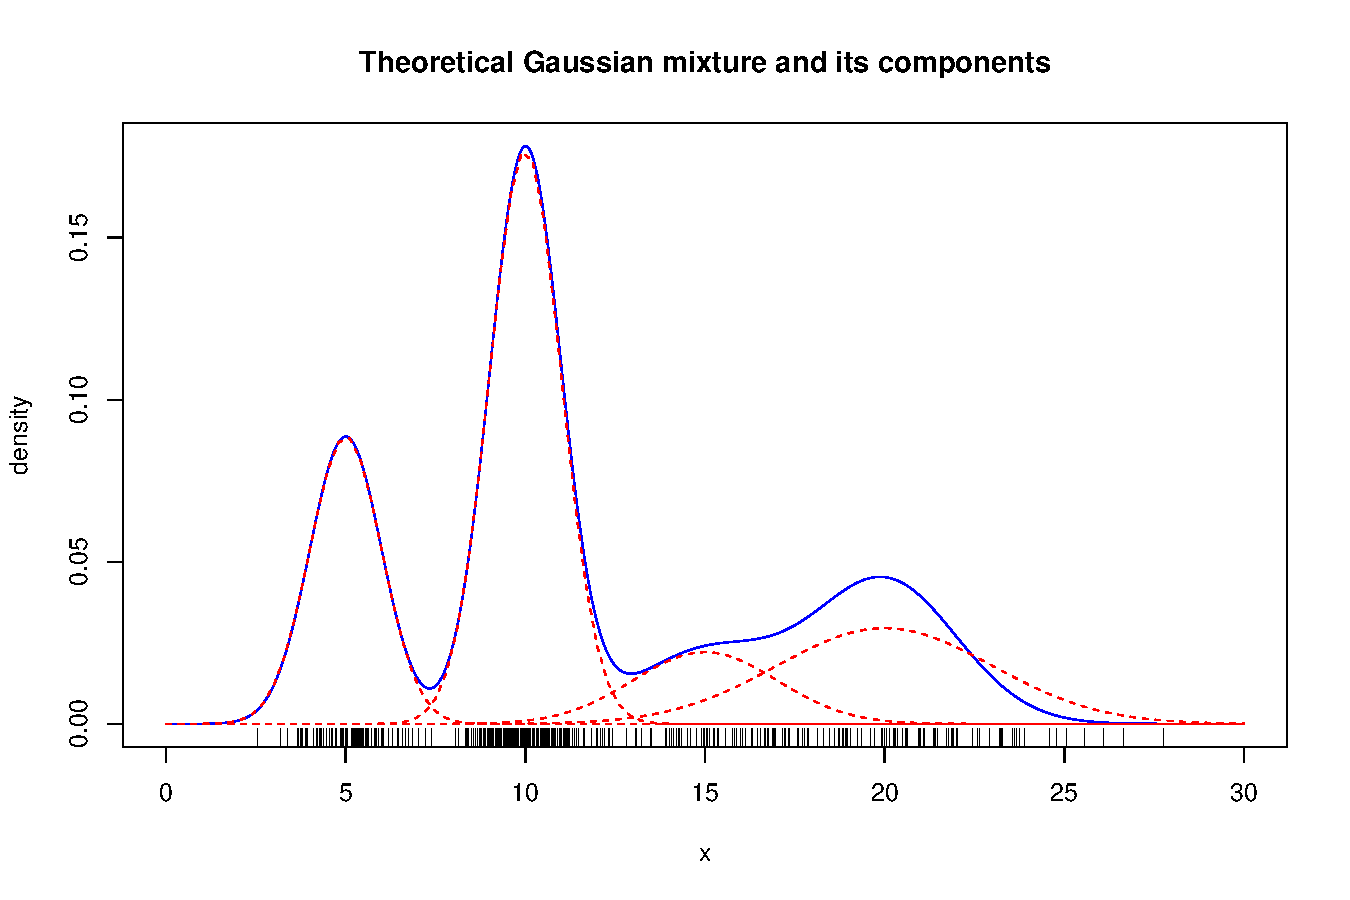
\includegraphics[width=.8\textwidth]{figures/EM_mixture_example_data_plot-1} 

\end{knitrout}
\end{frame}

\begin{frame}[fragile]
  \frametitle{Example: adjustment}

\begin{knitrout}\scriptsize
\definecolor{shadecolor}{rgb}{0.969, 0.969, 0.969}\color{fgcolor}\begin{kframe}
\begin{alltt}
\hlstd{out} \hlkwb{<-} \hlkwd{EM.mixture}\hlstd{(x,} \hlkwc{Q}\hlstd{=}\hlnum{4}\hlstd{,} \hlkwc{init.cl}\hlstd{=}\hlkwd{sample}\hlstd{(}\hlnum{1}\hlopt{:}\hlnum{4}\hlstd{,n,}\hlkwc{rep}\hlstd{=}\hlnum{TRUE}\hlstd{))}
\hlkwd{plot}\hlstd{(out}\hlopt{$}\hlstd{Eloglik,} \hlkwc{main}\hlstd{=}\hlstr{"EM criterion"}\hlstd{,} \hlkwc{type}\hlstd{=}\hlstr{"l"}\hlstd{,} \hlkwc{xlab}\hlstd{=}\hlstr{"iteration"}\hlstd{)}
\end{alltt}
\end{kframe}
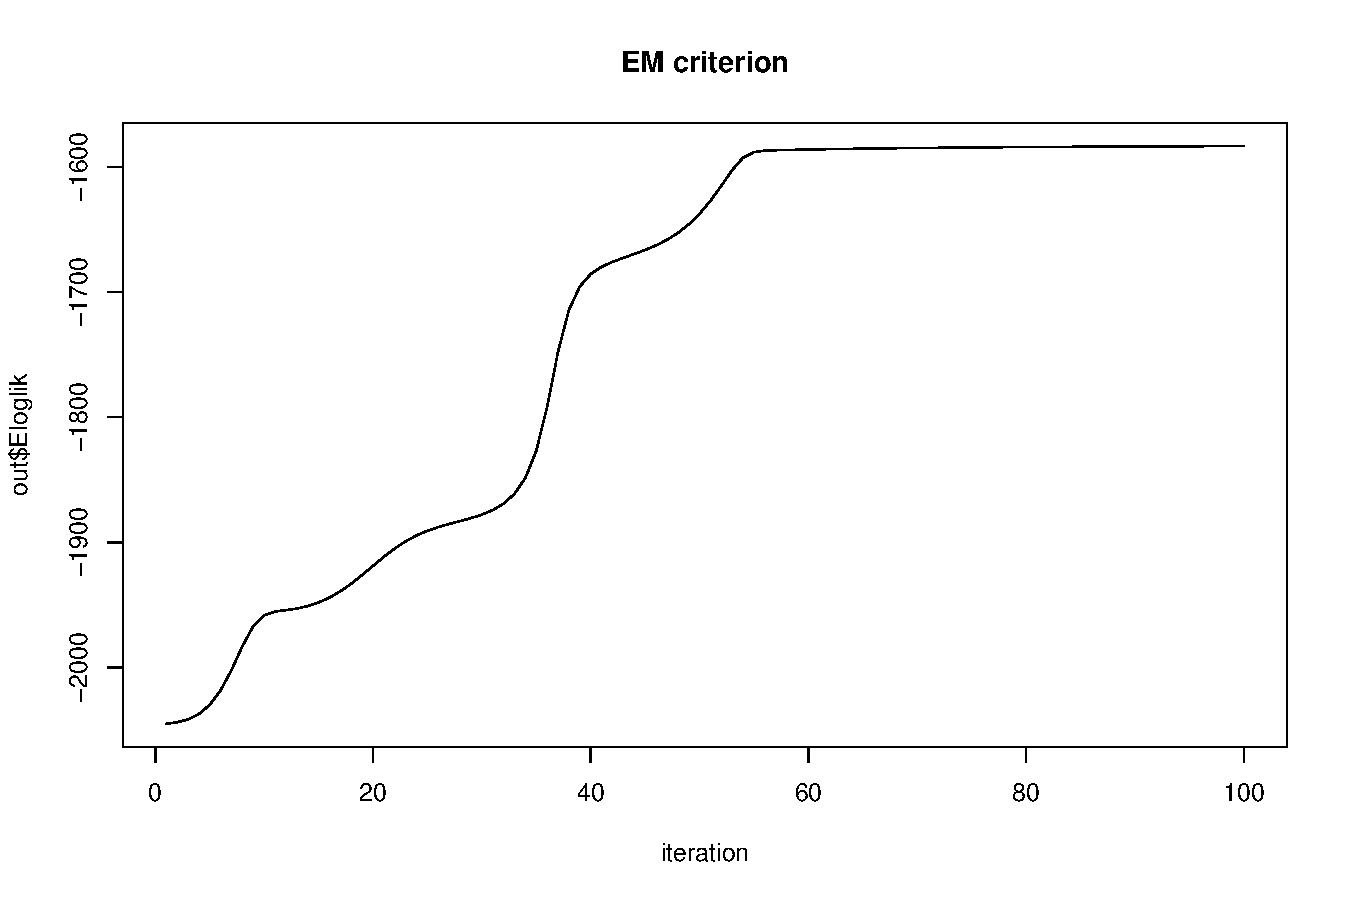
\includegraphics[width=.8\textwidth]{figures/EM_mixture_run-1} 

\end{knitrout}
\end{frame}

\begin{frame}[fragile, allowframebreaks]
  \frametitle{Example: adjustment - plot}

\begin{knitrout}\scriptsize
\definecolor{shadecolor}{rgb}{0.969, 0.969, 0.969}\color{fgcolor}\begin{kframe}
\begin{alltt}
\hlstd{out} \hlkwb{<-} \hlkwd{EM.mixture}\hlstd{(x,} \hlkwc{Q}\hlstd{=}\hlnum{4}\hlstd{,} \hlkwc{init.cl}\hlstd{=}\hlkwd{kmeans}\hlstd{(x,}\hlnum{4}\hlstd{)}\hlopt{$}\hlstd{cl)}
\hlkwd{curve}\hlstd{(alpha[}\hlnum{1}\hlstd{]}\hlopt{*}\hlkwd{dnorm}\hlstd{(x,mu1,sigma1)} \hlopt{+}
      \hlstd{alpha[}\hlnum{2}\hlstd{]}\hlopt{*}\hlkwd{dnorm}\hlstd{(x,mu2,sigma2)} \hlopt{+}
      \hlstd{alpha[}\hlnum{3}\hlstd{]}\hlopt{*}\hlkwd{dnorm}\hlstd{(x,mu3,sigma3)} \hlopt{+}
      \hlstd{alpha[}\hlnum{4}\hlstd{]}\hlopt{*}\hlkwd{dnorm}\hlstd{(x,mu4,sigma3),} \hlkwc{col}\hlstd{=}\hlstr{"blue"}\hlstd{,}
      \hlkwc{lty}\hlstd{=}\hlnum{1}\hlstd{,} \hlkwc{from}\hlstd{=}\hlnum{0}\hlstd{,}\hlkwc{to}\hlstd{=}\hlnum{30}\hlstd{,} \hlkwc{n}\hlstd{=}\hlnum{1000}\hlstd{,}
      \hlkwc{main}\hlstd{=}\hlstr{"Theoretical Gaussian mixture and estimated components"}\hlstd{,}
      \hlkwc{xlab}\hlstd{=}\hlstr{"x"}\hlstd{,} \hlkwc{ylab}\hlstd{=}\hlstr{"density"}\hlstd{)}
\hlkwd{curve}\hlstd{(out}\hlopt{$}\hlstd{alpha[}\hlnum{1}\hlstd{]}\hlopt{*}\hlkwd{dnorm}\hlstd{(x,out}\hlopt{$}\hlstd{mu[}\hlnum{1}\hlstd{],out}\hlopt{$}\hlstd{sigma[}\hlnum{1}\hlstd{]),} \hlkwc{col}\hlstd{=}\hlstr{"red"}\hlstd{,} \hlkwc{add}\hlstd{=}\hlnum{TRUE}\hlstd{,} \hlkwc{lty}\hlstd{=}\hlnum{2}\hlstd{)}
\hlkwd{curve}\hlstd{(out}\hlopt{$}\hlstd{alpha[}\hlnum{2}\hlstd{]}\hlopt{*}\hlkwd{dnorm}\hlstd{(x,out}\hlopt{$}\hlstd{mu[}\hlnum{2}\hlstd{],out}\hlopt{$}\hlstd{sigma[}\hlnum{2}\hlstd{]),} \hlkwc{col}\hlstd{=}\hlstr{"red"}\hlstd{,} \hlkwc{add}\hlstd{=}\hlnum{TRUE}\hlstd{,} \hlkwc{lty}\hlstd{=}\hlnum{2}\hlstd{)}
\hlkwd{curve}\hlstd{(out}\hlopt{$}\hlstd{alpha[}\hlnum{3}\hlstd{]}\hlopt{*}\hlkwd{dnorm}\hlstd{(x,out}\hlopt{$}\hlstd{mu[}\hlnum{3}\hlstd{],out}\hlopt{$}\hlstd{sigma[}\hlnum{3}\hlstd{]),} \hlkwc{col}\hlstd{=}\hlstr{"red"}\hlstd{,} \hlkwc{add}\hlstd{=}\hlnum{TRUE}\hlstd{,} \hlkwc{lty}\hlstd{=}\hlnum{2}\hlstd{)}
\hlkwd{curve}\hlstd{(out}\hlopt{$}\hlstd{alpha[}\hlnum{4}\hlstd{]}\hlopt{*}\hlkwd{dnorm}\hlstd{(x,out}\hlopt{$}\hlstd{mu[}\hlnum{4}\hlstd{],out}\hlopt{$}\hlstd{sigma[}\hlnum{4}\hlstd{]),} \hlkwc{col}\hlstd{=}\hlstr{"red"}\hlstd{,} \hlkwc{add}\hlstd{=}\hlnum{TRUE}\hlstd{,} \hlkwc{lty}\hlstd{=}\hlnum{2}\hlstd{)}
\hlkwd{rug}\hlstd{(x)}
\end{alltt}
\end{kframe}
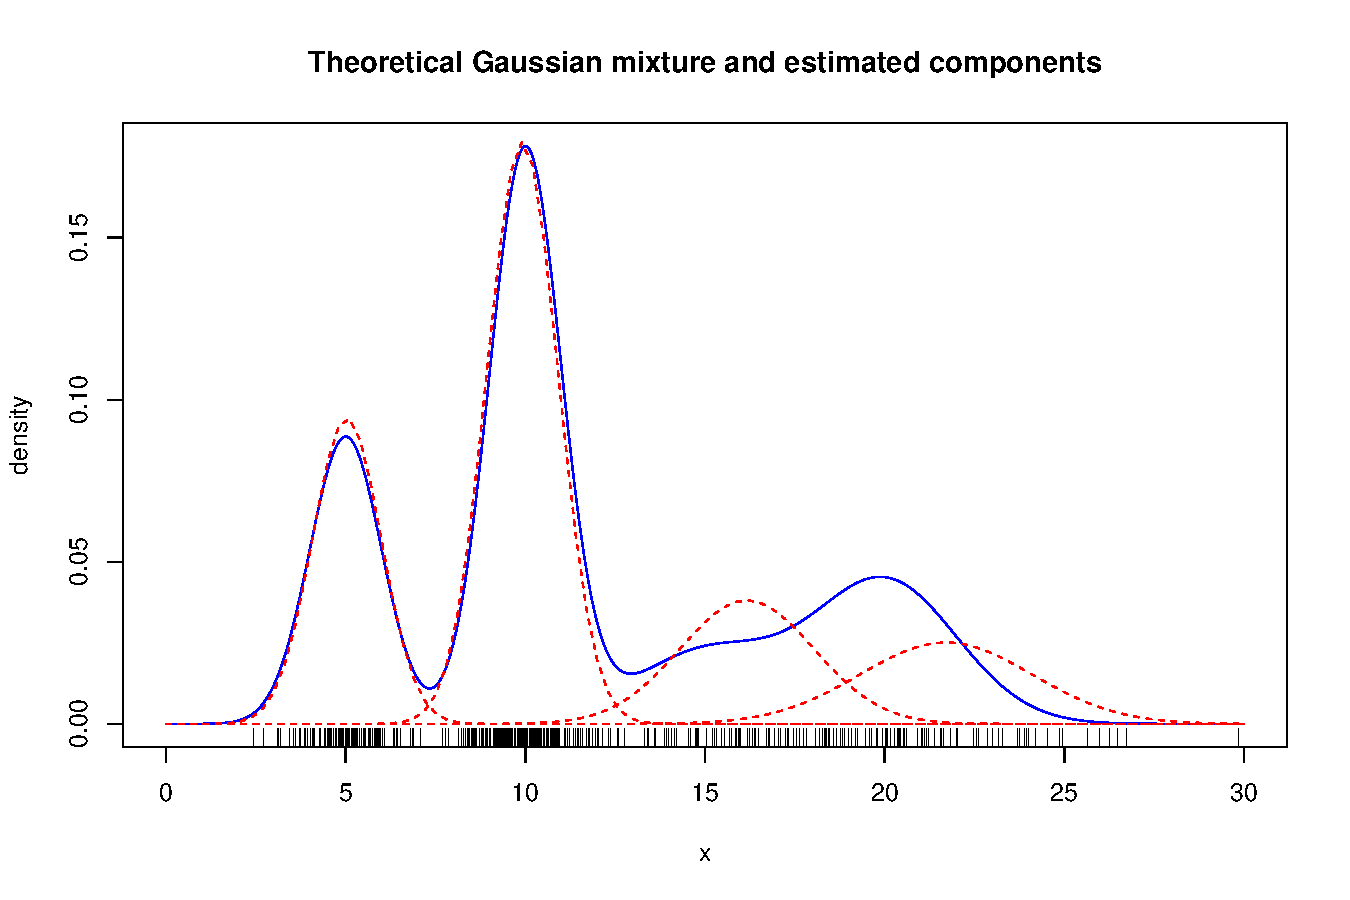
\includegraphics[width=.8\textwidth]{figures/EM_mixture_run_plot-1} 

\end{knitrout}

\end{frame}

\begin{frame}[fragile, allowframebreaks]
  \frametitle{Example: adjustment - classification}

\begin{knitrout}\scriptsize
\definecolor{shadecolor}{rgb}{0.969, 0.969, 0.969}\color{fgcolor}\begin{kframe}
\begin{alltt}
\hlkwd{table}\hlstd{(cl, out}\hlopt{$}\hlstd{cl)}
\end{alltt}
\begin{verbatim}
##    
## cl    1   2   3   4
##   1   0   0 100   0
##   2 197   1   2   0
##   3   2  45   0   3
##   4   0  36   0  64
\end{verbatim}
\begin{alltt}
\hlstd{aricode}\hlopt{::}\hlkwd{ARI}\hlstd{(cl, out}\hlopt{$}\hlstd{cl)}
\end{alltt}
\begin{verbatim}
## [1] 0.8686458
\end{verbatim}
\end{kframe}
\end{knitrout}

\end{frame}

%% ==========================================================================
\section{The Stochastic Block Model (SBM)}
%% ==========================================================================

\begin{frame}
  \frametitle{References}

    \begin{thebibliography}{99}
      \setbeamertemplate{bibliography item}[book]

    \bibitem[EK2]{EK2} Statistical Analysis of Network Data: Methods and Models
    \newblock \textcolor{black}{Eric Kolazcyk}
    \newblock \alert{Chapters 5 and 6}

      \setbeamertemplate{bibliography item}[article]

    \bibitem[EK2]{EK2} Mixture model for random graphs, Statistics and Computing
    \newblock \textcolor{black}{Daudin, Robin, Picard}
    \newblock {\tiny\url{pbil.univ-lyon1.fr/members/fpicard/franckpicard_fichiers/pdf/DPR08.pdf
}}

    \bibitem[CM1]{CM1} Analyse statistique de graphes,
    \newblock \textcolor{black}{Catherine Matias}
    \newblock \alert{Chapitre 4, Section 4}

    \end{thebibliography}

\end{frame}

%% ==========================================================================
\subsection{Some Graphs Models and their limitations}
%% ==========================================================================

\begin{frame}
  \frametitle{A mathematical model: Erdös-Rényi graph}

  \begin{definition}
    Let $\clV = {1,\dots,n}$ be a set of fixed vertices. The (simple) Erdös-Rény model $\mathcal{G}(n,\pi)$ assumes random edges between pairs of nodes with probability $\pi$. In orther word, the (random) adjacency matrix $\bX$ is such that
    \begin{equation*}
      X_{ij} \sim \mathcal{B}(\pi)
    \end{equation*}
  \end{definition}

  \vfill

  \begin{proposition}[degree distribution]
    The (random) degree $D_i$ of vertex $i$ follows a binomial distribution:
      \begin{equation*}
        D_i \sim b(n-1, \pi).
      \end{equation*}
  \end{proposition}

\end{frame}

\begin{frame}[fragile]
  \frametitle{Erdös-Rényi - example}

\begin{knitrout}\scriptsize
\definecolor{shadecolor}{rgb}{0.969, 0.969, 0.969}\color{fgcolor}\begin{kframe}
\begin{alltt}
\hlstd{G1} \hlkwb{<-} \hlstd{igraph}\hlopt{::}\hlkwd{sample_gnp}\hlstd{(}\hlnum{10}\hlstd{,} \hlnum{0.1}\hlstd{)}
\hlstd{G2} \hlkwb{<-} \hlstd{igraph}\hlopt{::}\hlkwd{sample_gnp}\hlstd{(}\hlnum{10}\hlstd{,} \hlnum{0.9}\hlstd{)}
\hlstd{G3} \hlkwb{<-} \hlstd{igraph}\hlopt{::}\hlkwd{sample_gnp}\hlstd{(}\hlnum{100}\hlstd{,} \hlnum{.02}\hlstd{)}
\hlkwd{par}\hlstd{(}\hlkwc{mfrow}\hlstd{=}\hlkwd{c}\hlstd{(}\hlnum{1}\hlstd{,}\hlnum{3}\hlstd{))}
\hlkwd{plot}\hlstd{(G1,} \hlkwc{vertex.label}\hlstd{=}\hlnum{NA}\hlstd{) ;} \hlkwd{plot}\hlstd{(G2,} \hlkwc{vertex.label}\hlstd{=}\hlnum{NA}\hlstd{)}
\hlkwd{plot}\hlstd{(G3,} \hlkwc{vertex.label}\hlstd{=}\hlnum{NA}\hlstd{,} \hlkwc{layout}\hlstd{=layout.circle)}
\end{alltt}
\end{kframe}
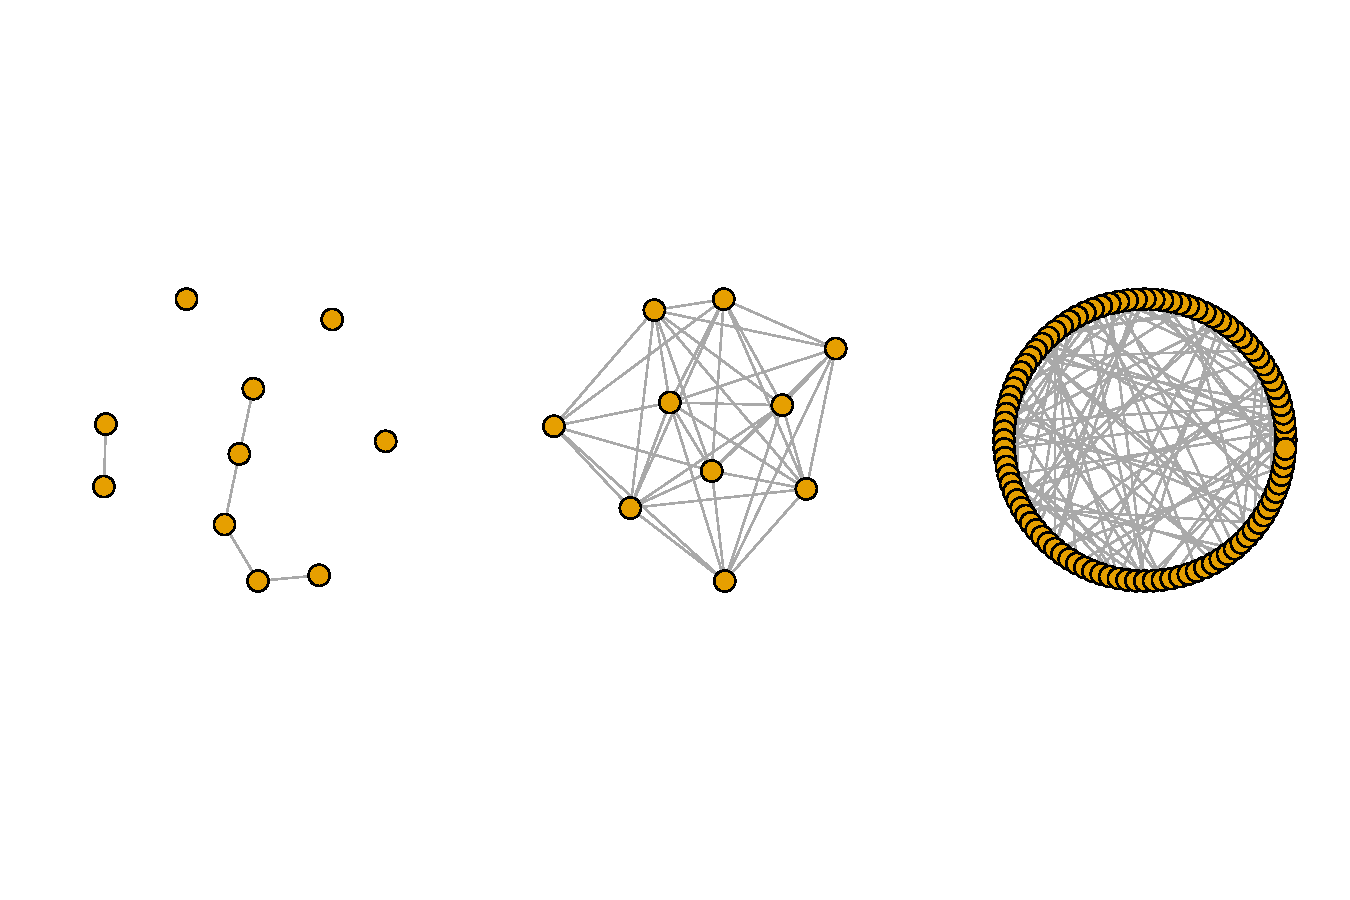
\includegraphics[width=.8\textwidth]{figures/ER_example-1} 

\end{knitrout}
\end{frame}

\begin{frame}[fragile]
  \frametitle{Erdös-Rény - limitations: very homegeneous}

\begin{knitrout}\scriptsize
\definecolor{shadecolor}{rgb}{0.969, 0.969, 0.969}\color{fgcolor}\begin{kframe}
\begin{alltt}
\hlkwd{average.path.length}\hlstd{(G3);} \hlkwd{diameter}\hlstd{(G3)}
\end{alltt}
\begin{verbatim}
## [1] 5.488342
## [1] 12
\end{verbatim}
\end{kframe}
\end{knitrout}

\begin{knitrout}\scriptsize
\definecolor{shadecolor}{rgb}{0.969, 0.969, 0.969}\color{fgcolor}
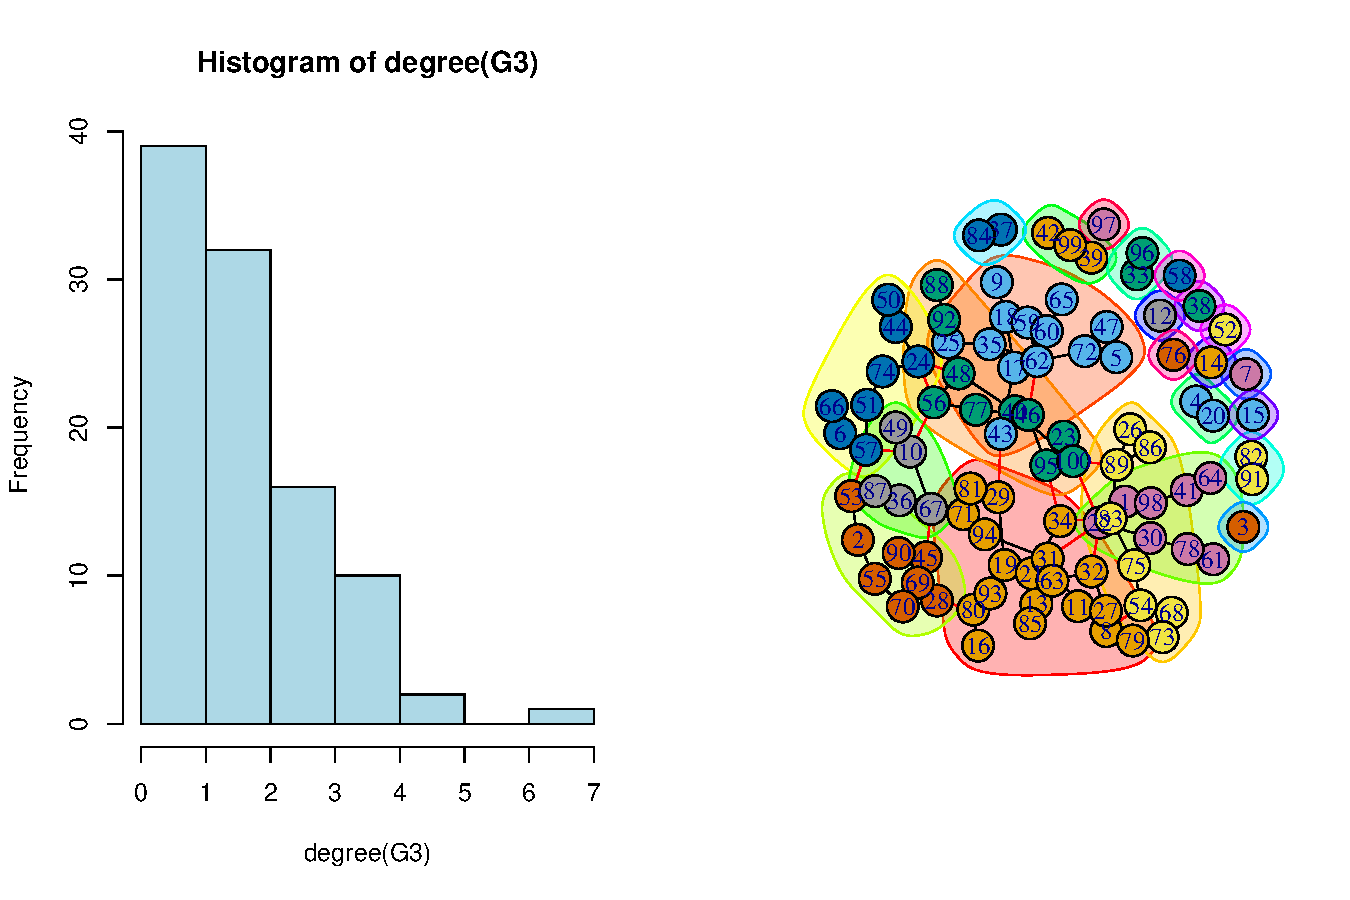
\includegraphics[width=.8\textwidth]{figures/ER_limitation2-1} 

\end{knitrout}
\end{frame}

\begin{frame}
  \frametitle{Mechanism-based model: preferential attachment}

  The graph is defined dynamically as follows
  \begin{block}{Definition}
    Start from a initial graph $\mathcal{G}_0 = (\mathcal{V}_0,\mathcal{E}_0)$, then for each time step,
    \begin{enumerate}
      \item At $t$ a new node $V_t$ is added
      \item $V_t$ is connected to $i \in V_{t-1}$ with probability
      \begin{equation*}
        D_i^\alpha + \mathrm{cst.}
      \end{equation*}
    \end{enumerate}
  \end{block}
  $\rightsquigarrow$ Nodes with high degree get more connections thus \alert{richers get richers}
\end{frame}

\begin{frame}[fragile]
  \frametitle{Preferential attachment - example}

\begin{knitrout}\scriptsize
\definecolor{shadecolor}{rgb}{0.969, 0.969, 0.969}\color{fgcolor}\begin{kframe}
\begin{alltt}
\hlstd{G1} \hlkwb{<-} \hlstd{igraph}\hlopt{::}\hlkwd{sample_pa}\hlstd{(}\hlnum{20}\hlstd{,} \hlnum{1}\hlstd{,} \hlkwc{directed}\hlstd{=}\hlnum{FALSE}\hlstd{)}
\hlstd{G2} \hlkwb{<-} \hlstd{igraph}\hlopt{::}\hlkwd{sample_pa}\hlstd{(}\hlnum{20}\hlstd{,} \hlnum{5}\hlstd{,} \hlkwc{directed}\hlstd{=}\hlnum{FALSE}\hlstd{)}
\hlstd{G3} \hlkwb{<-} \hlstd{igraph}\hlopt{::}\hlkwd{sample_pa}\hlstd{(}\hlnum{200}\hlstd{,} \hlkwc{directed}\hlstd{=}\hlnum{FALSE}\hlstd{)}
\hlkwd{par}\hlstd{(}\hlkwc{mfrow}\hlstd{=}\hlkwd{c}\hlstd{(}\hlnum{1}\hlstd{,}\hlnum{3}\hlstd{))}
\hlkwd{plot}\hlstd{(G1,} \hlkwc{vertex.label}\hlstd{=}\hlnum{NA}\hlstd{) ;} \hlkwd{plot}\hlstd{(G2,} \hlkwc{vertex.label}\hlstd{=}\hlnum{NA}\hlstd{)}
\hlkwd{plot}\hlstd{(G3,} \hlkwc{vertex.label}\hlstd{=}\hlnum{NA}\hlstd{,} \hlkwc{layout}\hlstd{=layout.circle)}
\end{alltt}
\end{kframe}
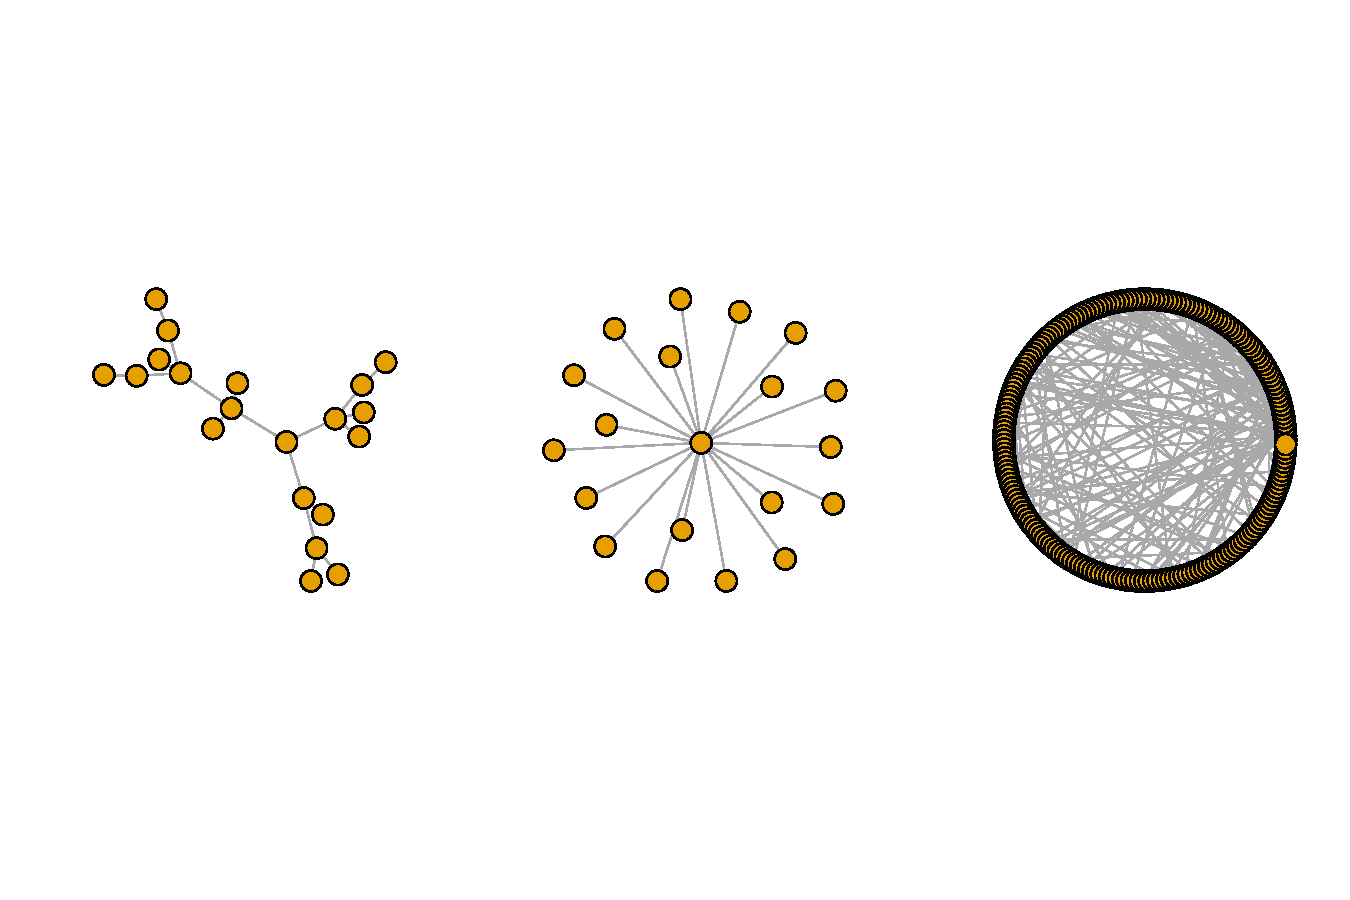
\includegraphics[width=.8\textwidth]{figures/PA_example-1} 

\end{knitrout}

\end{frame}

\begin{frame}[fragile]
  \frametitle{Preferential attachment - limitations}

\begin{knitrout}\scriptsize
\definecolor{shadecolor}{rgb}{0.969, 0.969, 0.969}\color{fgcolor}\begin{kframe}
\begin{alltt}
\hlkwd{average.path.length}\hlstd{(G3);} \hlkwd{diameter}\hlstd{(G3)}
\end{alltt}
\begin{verbatim}
## [1] 6.098844
## [1] 14
\end{verbatim}
\end{kframe}
\end{knitrout}

\begin{knitrout}\scriptsize
\definecolor{shadecolor}{rgb}{0.969, 0.969, 0.969}\color{fgcolor}
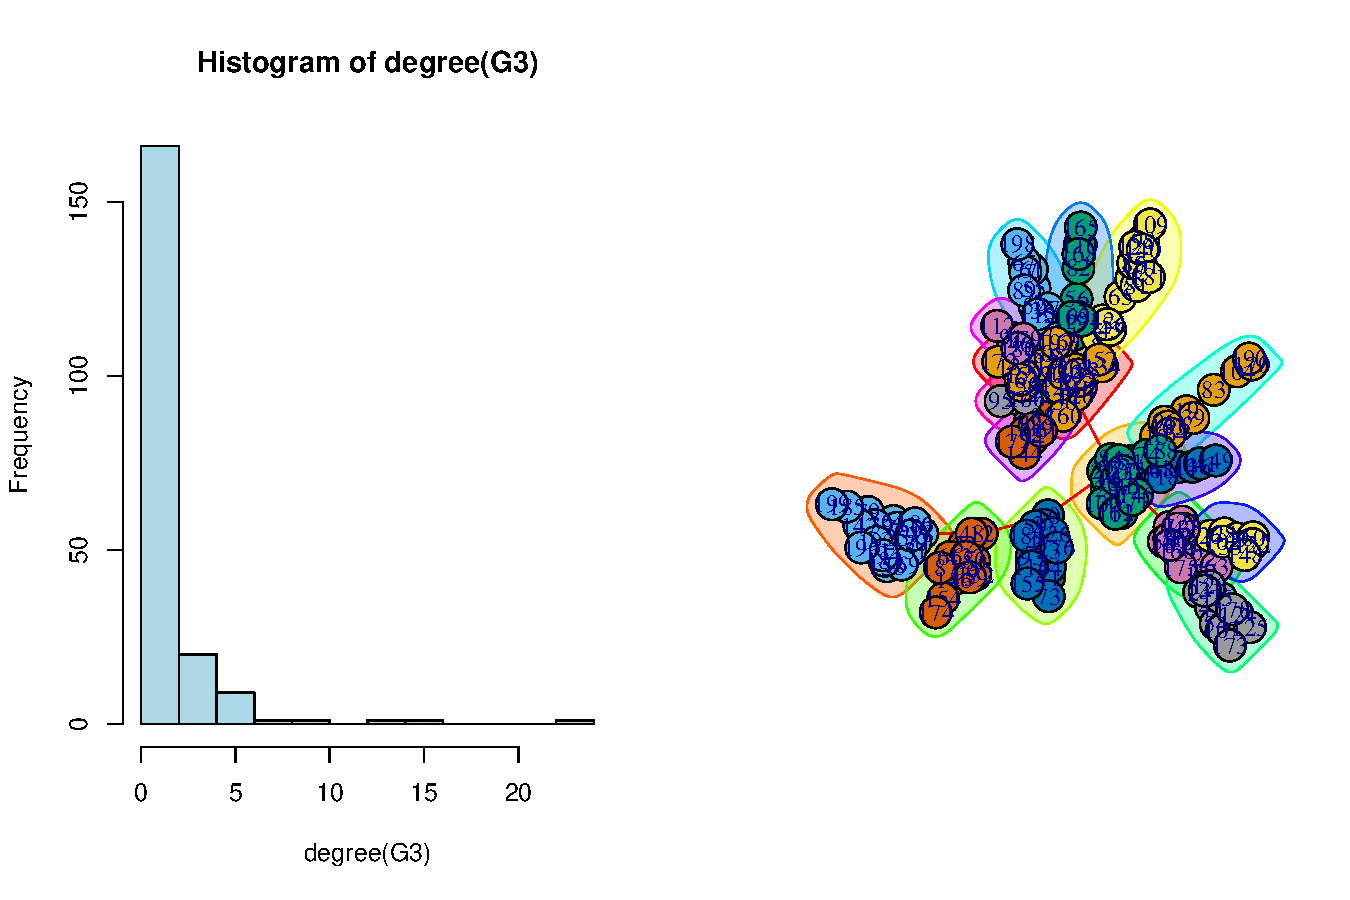
\includegraphics[width=.8\textwidth]{figures/PA_limitation2-1} 

\end{knitrout}
\end{frame}

\begin{frame}
  \frametitle{Limitations}

    \begin{itemize}
    \item \alert{Erdös-Rényi}\\
      The ER model does not fit well real world network
      \begin{itemize}
        \item As can been seen from its degree distribution
        \item ER is generally too homogeneous
      \end{itemize}
    \item \alert{Preferential attachment}
      \begin{itemize}
        \item Is defined through an algorithm so performing statistics is complicated
        \item Is stucked to the power-law distribution of degrees
      \end{itemize}
    \end{itemize}

  \vfill

  \begin{block}{The Stochastic Block Model}
    The SBM\footnote{Other models exist (e.g. exponential model for random graphs) but less popular.} generalizes ER in a mixture framework. It provides
    \begin{itemize}
      \item a statistical framework to adjust and interpret the parameters
      \item a flexible yet simple specification that fits many existing network data
    \end{itemize}
  \end{block}

\end{frame}


%% ==========================================================================
\subsection{Mixture of Erdös-Rényi and the SBM}
%% ==========================================================================

\begin{frame}
  \frametitle{Stochastic Block Model: definition}
    \framesubtitle{Mixture model point of view: mixture of Erdös-Rényi}

    \begin{block}{Latent structure}
      Let $\mathcal{V} = \set{1,..,n}$ be a fixed set of vertices. We give each $i\in\mathcal{V}$ a \alert{latent label} among a set $\mathcal{Q}=\{1,\dots,Q\}$ such that
    \begin{itemize}
    \item $\alpha_q = \prob(i\in q), \quad \sum_q \alpha_q=1$;
    \item $Z_{iq}=\1_{\{i \in  q\}}$  are independent  hidden variables.
   \end{itemize}
   \end{block}

    \begin{block}{The conditional distribution of the edges}
    Connexion probabilities depend on the node class belonging:
    \begin{equation*}
      X_{ij} | \set{i\in q, j\in\ell} \sim \mathcal{B}(\pi_{q \ell}) \qquad \bigg(\Leftrightarrow       X_{ij} | \set{Z_{iq}Z_{j\ell}=1} \sim \mathcal{B}(\pi_{q \ell}).
 \bigg)
    \end{equation*}
    The $Q\times Q$ matrix ${\boldsymbol\pi}$  gives for all couple of labels $\pi_{q\ell}=\mathbb{P}(X_{ij}=1|i\in q, j\in\ell)$.
   \end{block}

\end{frame}


\begin{frame}
  \frametitle{Stochastic Block Model: the big picture}

  \begin{center}
    \begin{overlayarea}{\textwidth}{.5\textheight}
      \begin{columns}
        \begin{column}{.45\paperwidth}
        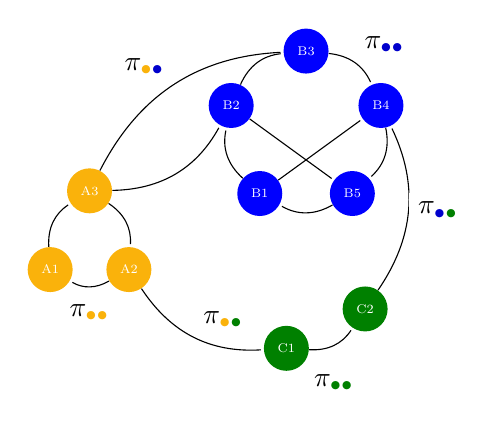
\begin{tikzpicture}
          %% UN GRAPH

          \tikzstyle{every edge}=[-,>=stealth',shorten >=1pt,auto,thin,draw]
          \tikzstyle{every state}=[draw=none,text=white,scale=0.65, font=\scriptsize, transform shape]
          \tikzstyle{every node}=[fill=yellow!40!orange]
          % premier cluster
          \node[state] (A1) at (0,0.5) {A1};
          \node[state] (A2) at (1,0.5) {A2};
          \node[state] (A3) at (.5,1.5) {A3};

          \path (A2) edge [bend left] node[fill=white,below=.1cm]
          {$\pi_{\textcolor{yellow!40!orange}{\bullet}\textcolor{yellow!40!orange}{\bullet}}$}
          (A1)
          (A1) edge [bend left] (A3)
          (A3) edge [bend left] (A2);

          \tikzstyle{every node}=[fill=blue!80!black]
          \foreach \angle/\text in {234/B1, 162/B2, 90/B3, 18/B4, -54/B5} {
            \node[fill=blue,state,xshift=5cm,yshift=3.5cm]     (\text)    at
            (\angle:1cm) {\text};
          }
          \path (B2) edge (B5)
          (B1) edge (B4);
          \foreach \from/\to in {1/2,2/3,4/5,5/1}{
            \path (B\from) edge [bend left] (B\to);
          }

          \path    (B3)    edge     [bend    left]    node[fill=white]
          {$\pi_{\textcolor{blue!80!black}{\bullet}\textcolor{blue!80!black}{\bullet}}$}  (B4) ;

          \tikzstyle{every node}=[fill=green!50!black]
          % troisieme cluster
          \node[state] (C1) at (3,-.5) {C1};
          \node[state] (C2) at (4,0) {C2};

          \path (C1) edge [bend right] node[fill=white,below=.25cm]
          {$\pi_{\textcolor{green!50!black}{\bullet}\textcolor{green!50!black}{\bullet}}$}
          (C2);

          % inter cluster
          \path (A3) edge [bend right]  (B2)
          (A3)    edge    [bend    left]    node[fill=white]
          {$\pi_{\textcolor{yellow!40!orange}{\bullet}\textcolor{blue!80!black}{\bullet}}$}
          (B3)
          (C2) edge [bend right] node[fill=white,right]
          {$\pi_{\textcolor{blue!80!black}{\bullet}\textcolor{green!50!black}{\bullet}}$}
          (B4)
          (A2) edge [bend right] node[fill=white]
          {$\pi_{\textcolor{yellow!40!orange}{\bullet}\textcolor{green!50!black}{\bullet}}$}
          (C1);
        \end{tikzpicture}
        \end{column}
        \begin{column}{.5\paperwidth}
          \begin{small}
            \begin{block}{Stochastic Block Model}
              Let $n$ nodes divided into
              \begin{itemize}
              \item
                $\mathcal{Q}=\{\textcolor{yellow!40!orange}{\bullet},\textcolor{blue!80!black}{\bullet},\textcolor{green!50!black}{\bullet}\}$
                classes
              \item  $\alpha_\bullet  =  \mathbb{P}(i  \in  \bullet)$,
                $\bullet\in\mathcal{Q},i=1,\dots,n$
              \item      $\pi_{\textcolor{yellow!40!orange}{\bullet}\textcolor{blue!80!black}{\bullet}}     =      \mathbb{P}(i
                \leftrightarrow j | i\in\textcolor{yellow!40!orange}{\bullet},j\in\textcolor{blue!80!black}{\bullet})$
              \end{itemize}
            \end{block}
          \end{small}
        \end{column}
      \end{columns}
    \end{overlayarea}
  \end{center}

  \begin{align*}
    Z_i = \mathbf{1}_{\{i \in \bullet\}}  \ & \sim^{\text{iid}} \mathcal{M}(1,\alpha), \quad \forall\bullet\in\mathcal{Q}, \\
    X_{ij} \ | \ \{i\in\textcolor{yellow!40!orange}{\bullet},j\in\textcolor{blue!80!black}{\bullet}\} & \sim^{\text{ind}} \mathcal{B}(\pi_{\textcolor{yellow!40!orange}{\bullet}\textcolor{blue!80!black}{\bullet}})\\
  \end{align*}

\end{frame}

\begin{frame}
  \frametitle{Stochastic Block Model: unknown parameters}

    \begin{center}
  \begin{overlayarea}{\textwidth}{.5\textheight}
      \begin{columns}
        \begin{column}{.45\paperwidth}
        \begin{tikzpicture}
          %% UN GRAPH

          \tikzstyle{every edge}=[-,>=stealth',shorten >=1pt,auto,thin,draw]
          \tikzstyle{every state}=[draw=none,text=white,scale=0.65, font=\scriptsize, transform shape]
          \tikzstyle{every node}=[fill=gray]
          % premier cluster
          \node[state] (A1) at (0,0.5) {N1};
          \node[state] (A2) at (1,0.5) {N2};
          \node[state] (A3) at (.5,1.5) {N3};

          \path (A2) edge [bend left] node[fill=white,below=.1cm]
          {}
          (A1)
          (A1) edge [bend left] (A3)
          (A3) edge [bend left] (A2);

          \tikzstyle{every node}=[fill=blue!80!black]
          \foreach \angle/\text in {234/N1, 162/N2, 90/N3, 18/N4, -54/N5} {
            \node[fill=gray,state,xshift=5cm,yshift=3.5cm]     (\text)    at
            (\angle:1cm) {\text};
          }
          \path (B2) edge (B5)
          (B1) edge (B4);
          \foreach \from/\to in {1/2,2/3,4/5,5/1}{
            \path (B\from) edge [bend left] (B\to);
          }

          \path (B3) edge [bend left] node[fill=white] {}  (B4) ;

          \tikzstyle{every node}=[fill=gray]
          % troisime cluster
          \node[state] (C1) at (3,-.5) {N1};
          \node[state] (C2) at (4,0) {N2};

          \path (C1) edge [bend right] (C2);

          % inter cluster
          \path (A3) edge [bend right]  (B2)
          (A3)    edge    [bend    left]    node[fill=white]
          {}
          (B3)
          (C2) edge [bend right] node[fill=white,right]
          {}
          (B4)
          (A2) edge [bend right] node[fill=white]
          {}
          (C1);
        \end{tikzpicture}
        \end{column}
        \begin{column}{.5\paperwidth}
          \begin{small}
            \begin{block}{Stochastic Block Model}
              Let $n$ nodes divided into
              \begin{itemize}
              \item
                $\mathcal{Q}=\{\textcolor{yellow!40!orange}{\bullet},\textcolor{blue!80!black}{\bullet},\textcolor{green!50!black}{\bullet}\}$,
                $\text{card}(\mathcal{Q})$ known
              \item  $\alpha_\bullet  =  ?$,
              \item      $\pi_{\textcolor{yellow!40!orange}{\bullet}\textcolor{blue!80!black}{\bullet}}     =      ?$
              \end{itemize}
            \end{block}
          \end{small}
        \end{column}
      \end{columns}
    \end{overlayarea}
    \end{center}

  \begin{align*}
    Z_i = \mathbf{1}_{\{i \in \bullet\}}  \ & \sim^{\text{iid}} \mathcal{M}(1,\alpha), \quad \forall\bullet\in\mathcal{Q}, \\
    X_{ij} \ | \ \{i\in\textcolor{yellow!40!orange}{\bullet},j\in\textcolor{blue!80!black}{\bullet}\} & \sim^{\text{ind}} \mathcal{B}(\pi_{\textcolor{yellow!40!orange}{\bullet}\textcolor{blue!80!black}{\bullet}})\\
  \end{align*}

\end{frame}

\begin{frame}[fragile]
  \frametitle{Stochastic block models -- examples of topology}
  \framesubtitle{Community network}

\begin{knitrout}\scriptsize
\definecolor{shadecolor}{rgb}{0.969, 0.969, 0.969}\color{fgcolor}\begin{kframe}
\begin{alltt}
\hlstd{pi} \hlkwb{<-} \hlkwd{matrix}\hlstd{(}\hlkwd{c}\hlstd{(}\hlnum{0.3}\hlstd{,}\hlnum{0.02}\hlstd{,}\hlnum{0.02}\hlstd{,}\hlnum{0.02}\hlstd{,}\hlnum{0.3}\hlstd{,}\hlnum{0.02}\hlstd{,}\hlnum{0.02}\hlstd{,}\hlnum{0.02}\hlstd{,}\hlnum{0.3}\hlstd{),}\hlnum{3}\hlstd{,}\hlnum{3}\hlstd{)}
\hlstd{communities} \hlkwb{<-} \hlstd{igraph}\hlopt{::}\hlkwd{sample_sbm}\hlstd{(}\hlnum{100}\hlstd{, pi,} \hlkwd{c}\hlstd{(}\hlnum{25}\hlstd{,} \hlnum{50}\hlstd{,} \hlnum{25}\hlstd{))}
\hlkwd{plot}\hlstd{(communities,} \hlkwc{vertex.label}\hlstd{=}\hlnum{NA}\hlstd{,} \hlkwc{vertex.color} \hlstd{=} \hlkwd{rep}\hlstd{(}\hlnum{1}\hlopt{:}\hlnum{3}\hlstd{,}\hlkwd{c}\hlstd{(}\hlnum{25}\hlstd{,} \hlnum{50}\hlstd{,} \hlnum{25}\hlstd{)))}
\end{alltt}
\end{kframe}
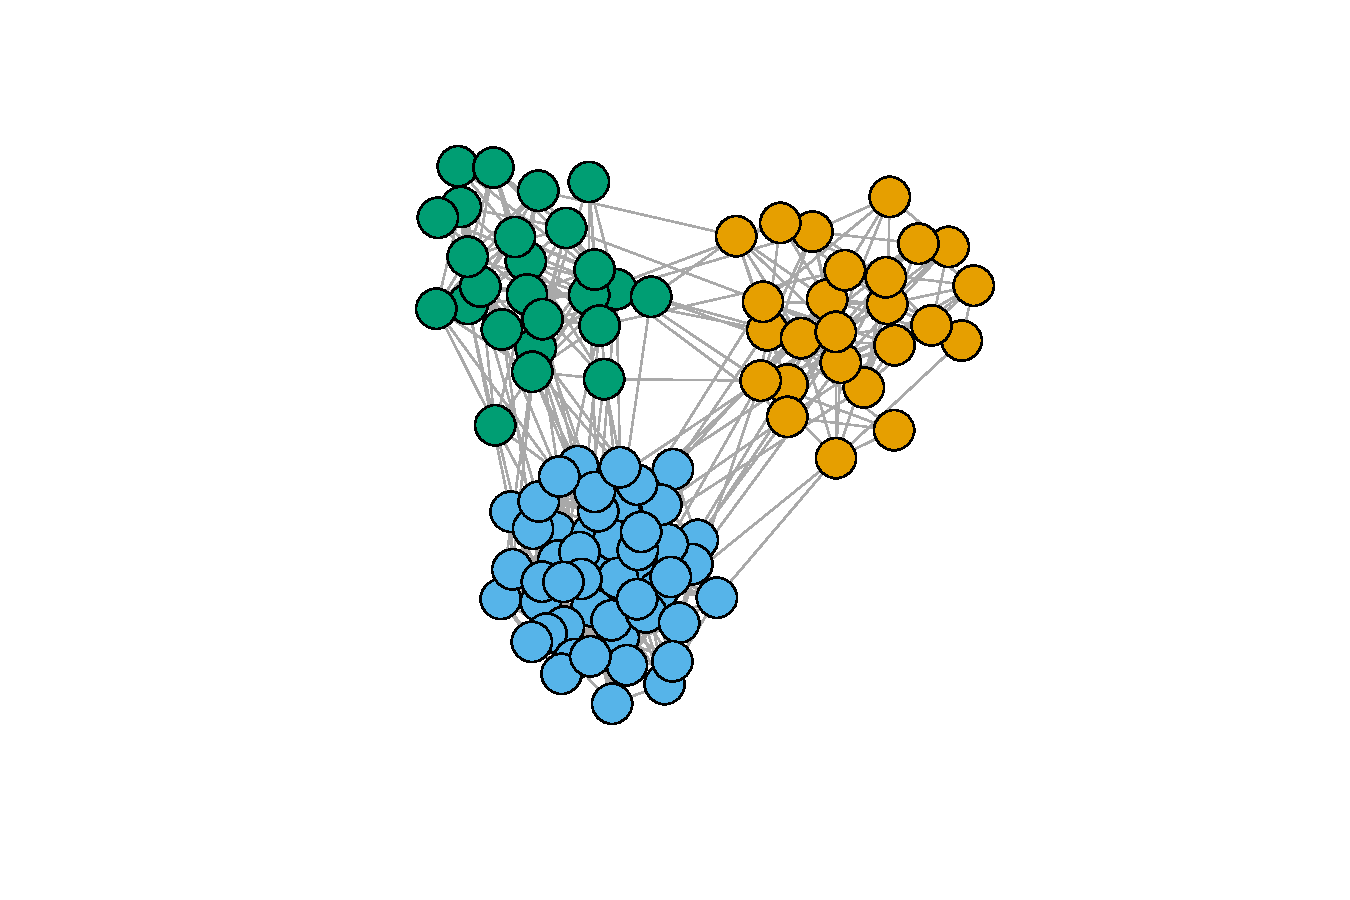
\includegraphics[width=.8\textwidth]{figures/unnamed-chunk-1-1} 

\end{knitrout}

\end{frame}

\begin{frame}[fragile]
  \frametitle{Stochastic block models -- examples of topology}
  \framesubtitle{Star network}

\begin{knitrout}\scriptsize
\definecolor{shadecolor}{rgb}{0.969, 0.969, 0.969}\color{fgcolor}\begin{kframe}
\begin{alltt}
\hlstd{pi} \hlkwb{<-} \hlkwd{matrix}\hlstd{(}\hlkwd{c}\hlstd{(}\hlnum{0.05}\hlstd{,}\hlnum{0.3}\hlstd{,}\hlnum{0.3}\hlstd{,}\hlnum{0}\hlstd{),}\hlnum{2}\hlstd{,}\hlnum{2}\hlstd{)}
\hlstd{star} \hlkwb{<-} \hlstd{igraph}\hlopt{::}\hlkwd{sample_sbm}\hlstd{(}\hlnum{100}\hlstd{, pi,} \hlkwd{c}\hlstd{(}\hlnum{4}\hlstd{,} \hlnum{96}\hlstd{))}
\hlkwd{plot}\hlstd{(star,} \hlkwc{vertex.label}\hlstd{=}\hlnum{NA}\hlstd{,} \hlkwc{vertex.color} \hlstd{=} \hlkwd{rep}\hlstd{(}\hlnum{1}\hlopt{:}\hlnum{2}\hlstd{,}\hlkwd{c}\hlstd{(}\hlnum{4}\hlstd{,}\hlnum{96}\hlstd{)))}
\end{alltt}
\end{kframe}
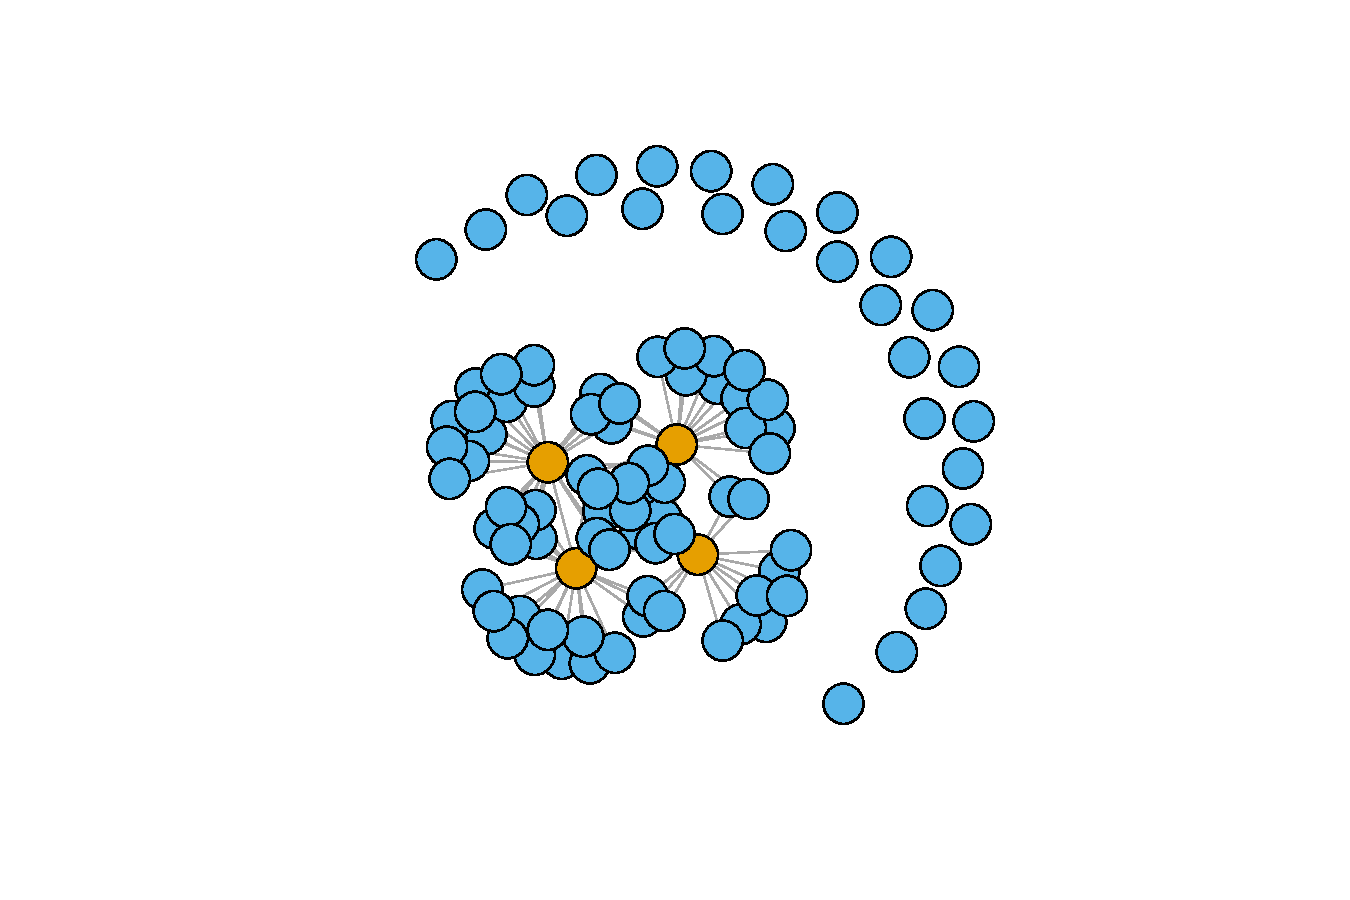
\includegraphics[width=.8\textwidth]{figures/unnamed-chunk-2-1} 

\end{knitrout}

\end{frame}

\begin{frame}
  \frametitle{Degree distributions}

  \begin{block}{Conditional degree distribution}
    The conditional degree distribution of a node $i\in q$ is
    \begin{equation*}
      D_i | i \in q \sim \mathrm{b}(n-1,\bar\pi) \approx \mathcal{P}(\lambda_q), \qquad \bar\pi_q = \sum_{\ell=1}^Q \alpha_\ell, \pi_{q\ell} \quad \lambda_q = (n-1)\bar\pi_q
    \end{equation*}
  \end{block}

  \vfill

  \begin{block}{Conditional degree distribution}
    The degree distribution of a node $i$ can be approximated by a mixture of Poisson distributions:
    \begin{equation*}
      \prob(D_i = k) = \sum_{q=1}^Q\alpha_q \exp{\set{-\lambda_q}} \ \frac{\lambda_q^k}{k !}
    \end{equation*}
  \end{block}

\end{frame}

\begin{frame}
  \frametitle{Likelihoods}

  \begin{block}{Complete-data loglikelihood}
    \vspace{-.5cm}
    \begin{equation*}
      \log L(\bX,\bZ) = \sum_{i,q} Z_{iq} \log \alpha_q + \sum_{i<j,q,\ell} Z_{iq}Z_{j\ell} \log \pi_{q\ell}^{X_{ij}} (1-\pi_{q\ell})^{1-X_{ij}}.
    \end{equation*}
  \end{block}

  \begin{block}{Conditional expectation of the complete-data loglikelihood}
    \vspace{-.5cm}
    \begin{equation*}
      \E_{\bZ|\bX} \big[\log L(\btheta;\bX,\bZ) \big] = \sum_{i,q} \tau_{iq} \log \alpha_q + \sum_{i<j,q,\ell} \eta_{ijq\ell} \log \pi_{q\ell}^{X_{ij}} (1-\pi_{q\ell})^{1-X_{ij}}
    \end{equation*}
      where $\tau_ {iq}, \eta_{ijq\ell}$ are the posterior probabilities:
      \begin{itemize}
        \item $\tau_{iq} = \prob(Z_{iq} = 1 | \bX) = \E \left[Z_{iq} | \bX\right].$
        \item $\eta_{ijq\ell} = \prob(Z_{iq}Z_{j\ell} = 1 | \bX) = \E \left[Z_{iq}Z_{j\ell} | \bX\right].$
      \end{itemize}
  \end{block}

\end{frame}

%% ==========================================================================
\subsection{Inference in SBM with variational EM}
%% ==========================================================================

\begin{frame}
  \frametitle{The EM strategy does not apply directly for SBM}

  \begin{block}{Ouch: another intractability problem}
    \begin{itemize}
      \item the $Z_{iq}$ are \alert{not independent} in the SBM framework\dots
      \item we cannot compute $\eta_{ijq\ell} = \prob(Z_{iq}Z_{j\ell} = 1 | \bX) = \E \left[Z_{iq}Z_{j\ell} | \bX\right]$,
      \item the conditional expectation $Q(\btheta)$, i.e. the main EM ingredient, is \alert{intractable}.
    \end{itemize}
  \end{block}

  \vfill

  \begin{block}{Solution: mean field approximation}
    Approximate $\eta_{ijq\ell}$ by $\tau_{iq}\tau_{j\ell}$, i.e., \alert{assume independence between $Z_{iq}$}\\

    $\rightsquigarrow$ This can be formalized in the variational framework
  \end{block}


\end{frame}

\begin{frame}
  \frametitle{Revisting the EM algorithm I}

  \begin{proposition}
    Consider a distribution $\mathbb{Q}$ for the $\set{Z_{iq}}$. We have
    \begin{equation*}
      \log L(\btheta; \bX) = \E_{\mathbb{Q}} [\log L(\btheta, \bX,\bZ)] + \mathcal{H}(\mathbb{Q}) + \mathrm{KL}(\mathbb{Q} \ | \ \prob(\bZ|\bX;\btheta)),
    \end{equation*}
    where $\mathcal{H}$ is the entropy and $\mathrm{KL}( \cdot| \cdot)$ is the Kullback-Leibler divergence:
    \begin{gather*}
      \mathcal{H}(\mathbb{Q}) = - \sum_z \mathbb{Q}(z) \log \mathbb{Q}(z) = - \E_\mathbb{Q} [\log \mathbb{Q} (Z)]\\
      \mathcal{KL}(\mathbb{Q} \ | \ \prob(\bZ|\bX;\btheta)) = \sum_z \mathbb{Q}(z) \log \frac{\mathbb{Q}(z)}{\prob(\bZ|\bX;\btheta)} = \E_\mathbb{Q} \left[\log \frac{\mathbb{Q}(z)}{\prob(\bZ|\bX;\btheta)}\right]\\
    \end{gather*}
  \end{proposition}
\end{frame}

\begin{frame}
  \frametitle{Revisting the EM algorithm II}
  Let
   \begin{equation*}
    J(\mathbb{Q},\btheta) \triangleq \E_{\mathbb{Q}}\left(\log L(\btheta ;\bX,\bZ)\right) + \mathcal{H}(\mathbb{Q})
\end{equation*}

  \vfill

  The steps in the EM algorithm may be viewed as:
  \begin{description}
    \item[Expectation step]: choose $\mathbb{Q}$ to maximize $J(\mathbb{Q};\btheta^{(t)})$\\[2ex]
      \alert{The solution is $\prob(\bZ|\bX;\btheta^{(t)})$}\\
    \item[Maximization step]: choose $\btheta$ to maximize $J(\mathbb{Q}^{(t)};\btheta$)\\[2ex]
      \alert{The solution maximizes $\E_{\bZ|\bX;\btheta^{(t)}}\left(\log L(\btheta ;\bX,\bZ)\right)$}
  \end{description}

\end{frame}

\begin{frame}
  \frametitle{Variational approximation for SBM}

    \begin{block}{Problem for SBM}
      $\prob(\bZ|\bX;\btheta^{(t)})$ cannot be computed thus the E-step cannot be solved.
  \end{block}

  \begin{block}{Idea}
      Choose $\mathbb{Q}$ in a class of function so that the E-step can be solved.
  \end{block}

  \begin{block}{Family of distribution that factorizes}
      We chose $\mathbb{Q}$ so as the $Z_{iq}$ are marginally independents:
      \begin{equation*}
        \mathbb{Q}(\bZ) = \prod_{i=1}^n \mathbb{Q}_i(Z_i) = \prod_{i=1}^n\prod_{q=1}^Q \tau_{iq}^{Z_{iq}},
      \end{equation*}
      where $\tau_{iq} =\mathbb{Q}_i(Z_{i} = q) = \E{Q}(Z_{iq})$, with $\sum_{q} \tau_{iq} = 1$ for all $i=1,\dots,n$.
  \end{block}

\end{frame}

\begin{frame}
  \frametitle{Variational EM for SBM: the criterion}

  \begin{block}{Lower bound of the loglikehood}
  Since $\mathbb{Q}$ is an approximation of $\prob(\bZ|\bX)$, the Kullback-Leibler divergence is non-negative and
    \begin{equation*}
      \log L(\btheta; \bX) \geq \E_{\mathbb{Q}} [\log L(\btheta, \bX,\bZ)] + \mathcal{H}(\mathbb{Q}) = J(\mathbb{Q},\btheta).
    \end{equation*}
  \end{block}

  For the SBM,
  \begin{equation*}
  J(\mathbb{Q},\btheta) = \sum_{i,q} \tau_{iq} \log \alpha_q + \sum_{i<j,q,\ell}  \tau_{iq}  \tau_{j\ell} \log b(X_{ij} ; \pi_{q\ell}) - \sum_{i,q} \tau_{iq} \log(\tau_{iq}),
  \end{equation*}

  $\rightsquigarrow$ we optimize the loglikelihood lower bound $J(\mathbb{Q},\btheta) = J(\boldsymbol\tau,\btheta)$ in $(\boldsymbol\tau, \btheta)$.

\end{frame}

\begin{frame}
  \frametitle{E and M steps for SBM}

  \begin{block}{Variational E-step}
    Maximizing $J(\boldsymbol\tau)$ for fixed $\btheta$, we find a fixed-point relationship:
    \begin{equation}
      \hat{\tau}_{iq} \varpropto \alpha_q \prod_{j} \prod_{\ell} b(X_{ij}, \pi_{q\ell})^{\hat{\tau}_{j\ell}}
    \end{equation}
  \end{block}

  \vfill

  \begin{block}{M-step}
    Maximizing $J(\btheta)$ for fixed $\boldsymbol\tau$, we find,
    \begin{equation}
\hat{\alpha}_q = \frac{1}{n}\sum_i \hat{\tau}_{iq} , \quad \hat\pi_{q\ell} = \frac{\sum_{i\neq j} \hat{\tau}_{iq}\hat{\tau}_{j\ell} X_{ij}}{\sum_{i\neq j} \hat{\tau}_{iq}\hat{\tau}_{j\ell}}.
\end{equation}
  \end{block}

\end{frame}

\begin{frame}
  \frametitle{Model selection}

  We use our lower bound of the  loglikelihood to compute an approximation of the ICL
  \begin{multline*}
  \mathrm{vICL}(Q) = \E_{\hat{\mathbb{Q}}} [\log L(\hat{\btheta)};\bX,\bZ] \\ - \frac{1}{2} \left(\frac{Q(Q+1)}{2} \log \frac{n(n-1)}{2} + (Q-1) \log (n) \right),
\end{multline*}
where
    \begin{equation*}
      \E_{\hat{\mathbb{Q}}} [\log L(\hat\btheta; \bX,\bZ)] = J(\hat{\boldsymbol\tau},\hat\btheta) - \mathcal{H}(\hat{\mathbb{Q}}).
    \end{equation*}

    The variational BIC is just
    \begin{equation*}
  \mathrm{vBIC}(Q) = J(\hat{\boldsymbol\tau},\hat\btheta) - \frac{1}{2} \left(\frac{Q(Q+1)}{2} \log \frac{n(n-1)}{2} + (Q-1) \log (n) \right).
    \end{equation*}

\end{frame}

\begin{frame}[fragile, allowframebreaks]
  \frametitle{Example on the French blogsphere}

\begin{knitrout}\scriptsize
\definecolor{shadecolor}{rgb}{0.969, 0.969, 0.969}\color{fgcolor}\begin{kframe}
\begin{alltt}
\hlkwd{library}\hlstd{(mixer)}
\hlkwd{data}\hlstd{(blog)}
\hlstd{mix.blog} \hlkwb{<-} \hlkwd{mixer}\hlstd{(}\hlkwc{x}\hlstd{=blog}\hlopt{$}\hlstd{links,}\hlkwc{qmin}\hlstd{=}\hlnum{2}\hlstd{,}\hlkwc{qmax}\hlstd{=}\hlnum{20}\hlstd{)}
\end{alltt}
\begin{verbatim}
## Mixer: the adjacency matrix has been transformed in a undirected edge list
\end{verbatim}
\begin{alltt}
\hlkwd{plot}\hlstd{(mix.blog)}
\end{alltt}
\end{kframe}
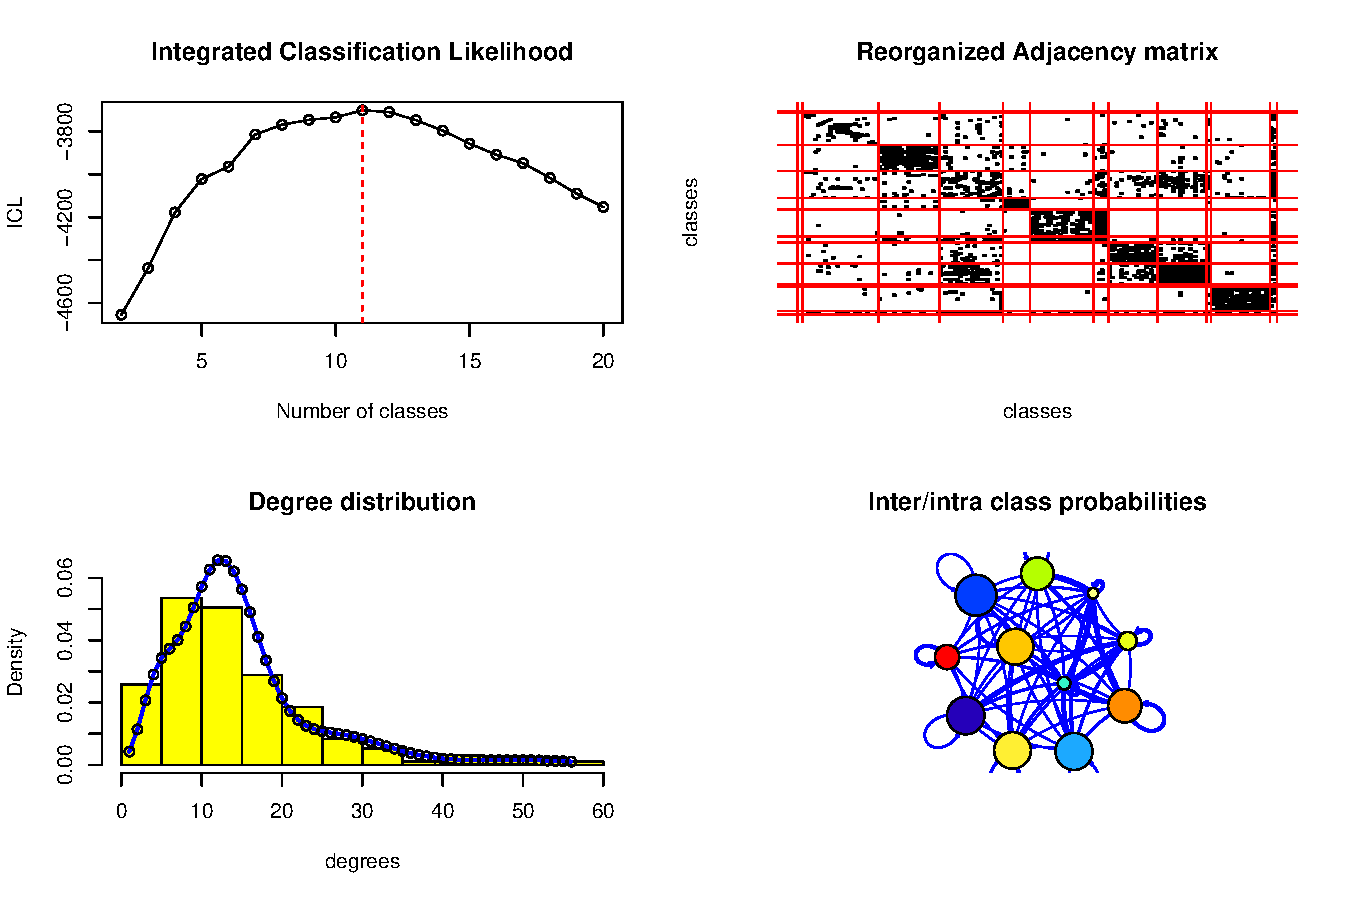
\includegraphics[width=.8\textwidth]{figures/example_mixer-1} 

\end{knitrout}

\end{frame}


\end{document}
